\documentclass[12pt]{article}
\usepackage{fontspec}
\usepackage{graphicx}
\usepackage{enumitem}
\usepackage{listings}
\usepackage{amsmath}
\usepackage{float}
\usepackage{algorithm}
\usepackage{algpseudocode}
\usepackage{indentfirst}
\usepackage{gensymb}
\usepackage{subfig}
\usepackage{url}
\usepackage[colorlinks=false]{hyperref}

\makeatletter
\g@addto@macro{\UrlBreaks}{\UrlOrds}
\makeatother

\algnewcommand\algorithmicforeach{\textbf{for each}}
\algdef{S}[FOR]{ForEach}[1]{\algorithmicforeach\ #1\ \algorithmicdo}

\setlength\parindent{2.5em}
%\setlength\parskip{0.5\baselineskip} 


\begin{document}
\setmainfont[Ligatures=TeX]{UTSans-Regular}

\tableofcontents
\newpage


\input{capitole/coperta.tex}
\newpage
\section{Cuvinte cheie}
\begin{itemize}
    \item Motion body - corp rigid, componentă a modelului 3D
    \item Joint - legătură într-un punct fix dintre două elemente Motion body
    \item Connector - element flexibil care leagă doua elemente Motion body, ex: un arc
    \item Mecanism - întregul model format din elemente Motion body, Joint și Connector
    \item .mdef - motion definition file, extensia fisierului care conține datele prelucrate de aplicație
    \item XML - extensible markup language
    \item C++ - limbaj de programare
    \item Qt - librarie grafica pentru C++
    \item Force-directed - clasa de algoritmi pentru desenarea grafurilor
\end{itemize}


\newpage
\section{Introducere}


În cartografie sau geologie, o hartă topologică este un tip de diagramă care conține doar informații esențiale. 
Numele este derivat din topologie, o ramură a matematicii care studiază proprietățile unui obiect care nu se schimba dacă 
obiectul în sine este deformat, fie prin întindere, îndoire, dar nu și rupere sau lipire. Aceste hărți nu au scară, iar distanța 
și direcția sunt supuse schimbării și variației, având în prim plan evidențierea relațiilor dintre anumite puncte esențiale. 
Un exemplu ar fi harta unui metrou care conține doar date importante precum numele stațiilor și ordinea lor, însa distanța 
dintre ele nu este întocmai cea din realitate. \newline

Acest concept este aplicat pentru crearea unei diagrame având la baza un model 3D format din mai multe elemente.
Modelul 3D este generat de aplicația de simulare Simcenter sub forma unui fisier .mdef care contine doar informații esențiale.
Aplicația prezentată în această lucrare are scopul de a vizualiza doar noțiuni semnificative precum relațiile dintre elemente
și tipul legăturilor lor. Această aplicație este necesară în cazurile când nu se dorește deschiderea întregului model în Simcenter
(lucru ce se dovedește ineficient în unele cazuri din punct de vedere al timpului de încărcare), ci doar crearea unei diagrame simple 
conținând caracteristicile prezentate anterior.\newline

\newpage
\section{Istorie}
Topologia, ca și o ramura  bine definita a matematicii, își are originile de la începutul secolului XX, 
însa au fost descoperite și cazuri izolate în aplicarea acestui concept chiar și cu câteva secole în urma. 
Leonhard Euler este considerat ca fiind primul care abordează acest domeniu prin lucrarea sa scrisa în 1736, 
Cele șapte poduri din Konigsberg, care se refera la crearea unui traseu prin oraș trecând peste fiecare pod o 
singura data., lucru ce sa dovedit imposibil.\newline

La 14 noiembrie 1750, Euler a scris unui prieten că a realizat importanța marginilor unui poliedru. 
Aceasta a condus la formula lui poliedrala: \[V-E+F=2\] unde V, E și F indică numărul de vârfuri, 
muchii și fețe ale poliedrului. Această analiză este considerata drept prima teoremă, semnalizând nașterea 
topologiei.\newline

Alte contribuții au fost făcute de Augustin-Louis Cauchy, Ludwig Schläfli, Johann Benedict Listing, 
Bernhard Riemann și Enrico Betti. Listing a introdus termenul "Topologie" în "Vorstudien zur Topologie", 
scris în limba germană, în 1847.\newline 

\newpage
\section{Graf}

Foarte multe probleme pot fi descrise printr-o diagrama formata dintr-un set de puncte și linii care conecteaza anumite perechi de puncte.
De exemplu, punctele pot reprezenta o multime de persoane, iar liniile dintre ele relatii de rudenie, sau punctele pot centre de comunicare 
iar liniile fiind legăturile dintre ele. Se poate observa ca in astfel de diagrame importanta este pusa pe modul in care sunt conectate acele puncte,
aspectul fiind nesemnificativ. O abstractie matematica a situatilor de acest tip este conceptul de graf.\newline

Un graf este o structură formată din obiecte în care sunt puse în evidență legăturile dintre ele. 
Obiectele corespund unor abstracții matematice numite, într-un graf, noduri/vârfuri (puncte) și fiecare legătură 
dintre perechile de obiecte asociate se numește muchie (arc sau linie). 
De obicei, un graf este reprezentat în formă schematică ca un set/grup de puncte care reprezintă nodurile, iar aceste sunt unite două 
câte două de linii sau curbe care corespund mulțimii muchiilor. Muchiile pot fi orientate/directe sau neorientate/indirecte.\newline

Grafurile sunt numite astfel datorită reprezentării grafice, și datorită acestei reprezentări putem înțelege proprietățile lor mult mai ușor.
Nu există un mod unic de desenare a unui graf; pozițiile relative ale punctelor care reprezintă nodurile si ale liniilor care reprezintă muchiile nu au importanță.\newline


Din punct de vedere matematic un graf G este un triplet ordonat \((V(G),E(E),\psi_g)\) care conține un set nevid \(V(G)\) de noduri, un set \(E(G)\),
disjunct de \(V(G)\), de muchii și o funcție de incidență \(\psi_G\) care asociază fiecarei muchii din \(G\) o pereche neordonata (dar nu neaparat distinctă)
de noduri din \(G\). Dacă \(e\) este o muchie și avem nodurile \(u\) și \(v\) astfel încât \(\psi_G(e)=uv\), atunci se spune că \(e\) unește \(u\) și \(v\); 
nodurile \(u\) și \(v\) sunt numite capetele lui \(e\).\newline

Majoritatea definițiilor și conceptelor în teoria grafurilor sunt sugerate de reprezentarea grafică. Capetele unei muchii sunt incidente cu muchia, si vice versa. 
Doua noduri care sunt incidente cu o muchie comună sunt adiacente, la fel pentru doua muchii care sunt incidente cu un nod comun. O muchie cu capete identice se numeste bucla.\newline

Un graf este finit dacă ambele seturi, cel de noduri și cel de muchii, sunt finite. Totodata un graf cu un singur nod se numește trivial, iar restul grafurilor netriviale.
Un graf este simplu dacă nu are bucle și nu există doua muchii care unesc aceleași două noduri.\newline

Doua noduri \(u\) și \(v\) sunt conexe daca exista un drum \((u,v)\) in \(G\), adică o secvența de noduri unice legate prin muchii care începe cu \(u\) și se termină cu \(v\).
Conectivitatea este o relație de chivalență pe setul de noduri \(V\). Astfel există o partiționare a lui \(V\) un subseturi nevide \(V_1,V_2,...V_n\) astfel încăt nodurile \(u\) și \(v\)
sunt conexe dacă și numai daca sunt din același set \(V_i\). Subgrafurile \(G[V_1], G[V_2], ... , G[V_n]\) se numesc componente ale lui \(G\). Dacă \(G\) are o singură componentă, atunci
\(G\) este conex, altfel este neconex.\newline

Ordinul unui graf reprezinta numărul de noduri, notat cu \(|V|\). Mărimea unui graf este numărul de muchii \(|E|\).
Gradul unui nod este numărul de muchii care sunt incidente cu el.
Într-un graf de ordin \(n\), gradul maxim al oricărui nod este de \(n-1\), iar numărul maxim de muchii este \(n(n-1)/2\).

\subsection{Multigraf}

Un multigraf este o generalizare în care oricare doua noduri pot avea mai multe muchii între ele. Acele muchii sunt numite și muchii paralele sau muchii multiple.
Exista doua noțiuni distincte despre muchii paralele:\newline

\begin{itemize}
\item Muchii fără identitate: identitatea unei muchii ține de cele doua noduri de care aparține. 
În unele cazuri nevoia de a distinge muchii multiple dintre doua noduri poate lipsi, iar acele muchii sunt considerate ca o 
singura entitate.\newline
\item Muchii cu identitate: în acest caz fiecare muchie este considerată ca fiind o primitiva, la fel ca nodurile, 
iar în cazul în care intre doua noduri exista mai multe muchii, fiecare dintre ele este considerata fiind o entitate distinctă.\newline
\end{itemize}

Definiție matematică:\newline

\begin{itemize}
\item Multigraf neorientat, cu muchii fara identitate: 
\(G=(V,E)\) unde:
\begin{itemize}
    \item \(V\) este un set de noduri 
    \item \(E\) este un multiset de perechi de noduri, numite muchii.
\end{itemize}

    
\item Multigraf neorientat, cu muchii cu identitate:
\(G=(V,E,r)\), unde:
\begin{itemize}
    \item \(V\) este un set de noduri
    \item \(E\) este un set de muchii
    \item \(r : E → \{\{x,y\} : x, y \in V\}\)
\end{itemize}

\end{itemize}

\subsection{Graf planar}

Un graf planar este un graf care poate fi încorporat într-un plan, adică un graf care poate fi desenat astfel încât 
marginile sale sa se intersecteze doar în noduri. Cu alte cuvinte, muchiile grafului sa nu se suprapună.\newline

Matematicianul polonez Kazimierz Kuratowski a caractetizat idea de graf planar prin următoarea teoremă:\newline

Un graf finit este planar dacă și numai dacă nu conține un subgraf care este o subdiviziune a grafului complet \(K_5\) sau a grafului complet bipartit \(K_{3,3}\).
O subdiviziune a unui graf rezulta din inserarea a oricâte noduri într-o muchie.\newline

O alta modalitate de a descrie un graf planar este prin teorema lui Wagner, exprimată în legătura cu noțiunea de graf minor:\newline
 
Un graf finit este planar dacă și numai dacă nu conține grafurile \(K_5\) sau \(K_{3,3}\) ca graf minor.
Un minor al unui graf rezulta prin contractarea unei muchii într-un nod, fiecare vecin al nodului original devenind vecin cu nodul nou.\newline

\begin{figure}[H]
    \begin{center}
        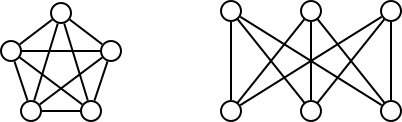
\includegraphics[scale=0.7]{imagini/graf/notplanar.png}        
    \end{center}
    \caption{Grafurile \(K_5\) si \(K_{3,3}\)}
    \label{fig:tabs}
\end{figure}

Alte criterii de planaritate:\newline
In practica este dificil sa folosim teorema lui Kuratowski pentru a decide într-un mod eficient dacă un graf este planar sau nu. 
Exista și alți algoritmi pentru rezolvarea acestei probleme, pentru un graf cu n noduri cu o complexitate de \(O(n)\).

Un graf simplu  cu \(v>=3\) noduri, \(e\) muchii și \(f\) fețe, trebuie sa îndeplinească următoarele condiții pentru a fi planar:
\begin{itemize}
    \item  \(e<=3v-6\)
    \item  dacă nu sunt cicluri de lungime \(3\), atunci \(e<=2v-4\) 
    \item  \(f<=2v-4\)
\end{itemize}

Formula lui Euler: \newline
Formula lui Euler afirmă că dacă un graf planar, finit, conectat, este desenat într-un plan și \(v\) este numărul de vârfuri, 
\(e\) este numărul de muchii și \(f\) este numărul de fețe (regiuni marcate de muchii , inclusiv regiunea exterioară, infinit de mare)
\[v-e+f=2\]

\begin{figure}[H]
    \begin{center}
        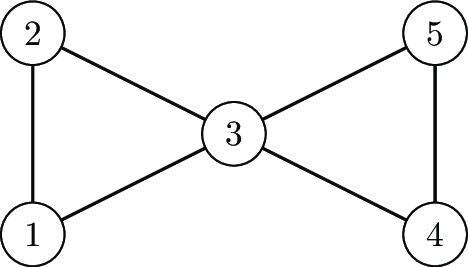
\includegraphics[scale=0.5]{imagini/graf/butterfly.png}
        \caption{Graf fluture}
        \label{fig:tabs}
    \end{center}    
\end{figure}


Ca o ilustrare, în graful fluture dat mai sus, \(v = 5\), \(e = 6\) și \(f = 3\). În general, dacă proprietatea este valida 
pentru toate grafurile planare cu \(f\) fețe, orice modificare a grafului care ar crea o față suplimentară, graful 
fiind în continuare planar ar fi și \(v - e + f\) invariant. Din moment ce proprietatea este valid pentru toate grafurile 
cu \(f = 2\), prin inducție matematică este valabilă pentru toate cazurile. Formula lui Euler poate fi demonstrata și în 
modul următor: dacă graful nu este un arbore, șterge o muchie care completează un ciclu. Astfel scade atât e, cât și 
\(f\) cu unul, lăsând \(v - e + f\) constantă. Repetați până când graficul rămas este un arbore; copacii au \(v = e + 1\) și \(f = 1\), 
producând \(v - e + f = 2\).\newline

\subsection{Aplicare}

Grafurile pot fi folosite pentru modelarea relațiilor și proceselor într-un sistem fizic, biologic, 
social sau informatic. Multe probleme practice pot fi reprezentate prin grafuri. In domeniul informaticii 
grafurile pot fi folosite pentru a reprezenta rețele de comunicare, organizarea datelor, dispozitive computerizate, 
fluxul de calcul, etc. De exemplu și un site web poate fi reprezentat printr-un graf, paginile web fiind nodurile 
iar legăturile dintre ele, link-urile, fiind muchiile. O abordare similara poate fi proiectate pentru multe alte domenii, 
precum ingineria mecanica unde putem exprima relațiile dintre mai multe elemente mecanice printr-un graf. Dezvoltarea 
algoritmilor pentru a gestiona grafuri este, prin urmare, de interes major în domeniul informaticii.











\newpage
\section{Algortimi force-directed de desenare a grafurilor}

Este o categorie de algoritmi de desenare a grafurilor într-un mod plăcut din punct de vedere estetic. 
Printr-un asftle de algoritm se positioneaza nodurile grafului într-un spațiu bidimensional sau tridimensional astfel încât 
lungimea muchiilor este mai mult sau mai puțin egală iar în structura grafului există un număr minim de suprapuneri intre muchii, 
iar în cazuri favorabile nici o suprapunere. Desenarea grafurilor poate fi o problema grea de abordat dar prin algoritmii 
de desenare force-directed, se exclud noțiuni ce țin de planaritatea grafurilor, întreaga operație de desenare fiind mai 
degrabă o simulare cu aspecte ce se regăsesc în fizică.\newline

Prin asignarea anumitor foțe setului de  noduri și setului de muchii din graf acestea fie se apropie fie se depărtează după 
fiecare iterație a algoritmului, scopul algoritmului fiind de a minimiza deplasarea nodurilor sau a muchiilor pana când se 
ajunge la o stare de echilibru. De obicei forțe elastice bazate pe legea lui Hooke sunt atribuite nodurilor unei muchii 
pentru ca acestea sa se atragă, în schimb ce simultan forte de repulsie, similare cu cele a particulelor cu sarcina electrică 
bazate pe legea lui Coulomb, sunt folosite pentru a crea o repulsie între nodurile grafului. In stările de echilibru al acestui sistem de forte, 
muchiile nodurilor care au un parinte comun au de obicei lungimea aproape egala (datorita forței elastice de atracție), 
iar nodurile care nu sunt conectare printr-o muchie se resping intre ele (datorita forței de repulsie). Fortele de atracție și repulsie pot fi definite și prin funcții 
care nu sunt bazate pe legile fizice ale elasticității sau sarcinii electrice, de exemplu unele sisteme pot folosi funcții de 
atracție logaritmice în loc de funcții liniare.\newline

O forță similară cu cea a gravitații poate fi folosită pentru a atrage nodurile către un punct fix în planul de desenare, 
astfel pentru un graf cu mai multe componente conexe acestea vor sta relativ în aceeași zonă și nu se vor mai depărta 
constant una de cealaltă datorita forței continue de repulsie și a lipsei de atracție intre ele. Forțe similare cu cele 
magnetice pot fi aplicate într-un sistem, atât pe noduri cât și pe muchii în sine pentru a evita suprapunerea muchiilor 
în întreaga simulare.\newline

\subsection{Aplicare}

Odată ce forțele au fost atribuite nodurilor sau muchiilor dintr-un graf întregul comportament al elementelor 
este simulat ca într-un sistem fizic unde nodurile se deplasează la fiecare iterație. Acest proces este repetat 
iterativ pana când se ajunge la o stare de echilibru mecanic, adică pozițiile relative ale elementelor nu se mai 
schimba de la o iterație la alta. Structura finala după întregul proces este folosită pentru a reprezenta graful ce 
trebuie desenat.\newline

Este posibilă și adăugarea unui mecanism de calculare a stării de echilibru pe lângă simularea fizică, acestea fiind 
metode de optimizare globala precum algoritmi genetici.\newline

\subsection{Avantaje}
\begin{itemize}
\item Rezultate calitative

Pentru grafuri de mărimi medii (50-500) de noduri de multe ori rezultatul aplicării unui algoritm force-directed este 
unul bun și inteligibil din perspectiva omului. Rezultatul fiind catalogat după următoarele criterii: 
\begin{itemize}
    \item lungimea uniforma a muchiilor
    \item distribuirea uniforma a nodurilor
    \item numar de supirapuneri minim
    \item simetrie
\end{itemize}

Simetria este un criteriu greu de îndeplinit și depinde de structura interna a grafului.
\item Flexibilitate

Algoritmul ales poate fi adaptat pentru a îndeplinii criterii adiționale de desenare. 
Exemple de extensibilitate are fi desenarea de: 
\begin{itemize}
    \item grafuri orientate
    \item grafuri 3D
    \item grafuri împărțite în clustere
    \item multigrafuri
    \item grafuri ponderate
\end{itemize}
\item Intuitivitate

Având la baza analogii din fizica, precum elasticitatea, comportamentul algoritmului este ușor de prezis și înțeles.
\item Simplitate

De obicei astfel de algoritmi sunt ușor de implementat, sau au fost deja implementati in anumite biblioteci.
\item Interactivitate

Prin desenarea unor stagii intermediare a grafului pe care este aplicat algoritmul, utilizatorul poate urmării evoluția 
procesului, observând cum se dezvolta dintr-o structura încurcata cu multe suprapuneri de muchii, într-un graf echilibrat 
și ușor de urmărit.
\item Fundatie teoretica 

Inca din anii 1960 metode de desenare ale grafurilor au fost cercetate, o prima implementare fiind făcuta 
prin algoritmul lui Tutte în anul 1963 folosind o reprezentare baricentrică (prin care se se seteaza un grup de noduri 
de baza în jurul cărora celelalte noduri vor fi plasate), folosind doar forte de atracție. 
In următorii ani alte metode de desenare au fost create de către Eades(1984), Fruchterman și Reingold (1991), Kamada și Kawai (1989).

\end{itemize}

\subsection{Dezavantaje}

\begin{itemize}
\item Timp de rulare mare

De obicei complexitatea unui algoritm de desenare force-directed este \(O(n^3)\), unde \(n\) este numărul de noduri din graf. 
Acest lucru rezulta deoarece numărul iterațiilor este estimat ca fiind \(O(n)\) iar pentru fiecare iterație fiecare 
pereche de noduri trebuie vizitata pentru calcularea forței de repulsie mutuale.

\item Minim local

Prin algoritmii force-directed se ajunge la o structura în care nodurile se afla într-o stare de echilibru, întreg procesul poate 
fi consideratca ca fiind rezolvarea unei probleme de optimizare.
De cele mai multe ori starea rezultata se poate afla într-un minim local al funcție ce trebuie optimizate, dar care nu 
coincide neapărat cu un minim global. Întreg procesul depinde de starea inițială a nodurilor care este aleasa aleatoriu. 
Aceasta problema creste odată cu numărul de noduri din graf. O modalitate de rezolvare ar fi combinarea a mai multor 
algoritmi force-directed pentru obținerea unui rezultat mai bun. De exemplu folosirea algoritmului Kamada–Kawai pentru 
crearea unei așezări în plan inițiale, iar apoi îmbunătățirea structurii cu ajutorul algoritmului Fruchterman–Reingold.

\end{itemize}

\subsection{Metode de desenare}
\subsubsection{Metoda baricentrică}
Metoda baricentrică de desenare a lui Tutte din 1963 este considerată prima versiune a unui algoritm force-directed 
pentru obținerea unei structuri cu muchii drepte, fără suprapuneri pentru un graf planar 3-conex. In comparație cu alte 
metode de desenare această varianta garantează ca fețele grafului planar sunt convexe. Idea în spatele algoritmului 
consta în faptul ca dacă o față a grafului planar este fixată în plan, atunci pozițiile potrivite a celorlalte noduri sunt 
găsite rezolvănd un set de ecuații liniare, unde fiecare poziția a unui nod este reprezentata ca o combinație convexa a 
pozițiilor nodurilor vecine lui. In acest model forța unei muchii \((u,v)\) este direct proporțională cu distanta dintre 
nodul \(u\) și \(v\) in plan. Astfel forța la un nod \(v\) este descrisa prin 
\[F(v)=\sum_{(u,v) \in E} p_u-p_v\] 
unde \(p_u\) și \(p_v\) sunt pozițiile nodurilor. Deoarece aceasta funcție are un minim cu toate nodurile așezate în aceeași locație, setul 
de noduri trebuie împărțit în noduri fixe și noduri libere, care pot fi deplasate.

\begin{algorithm}[H]
    \caption{Metoda baricentrică de desenare}
    Input: \(G=(V,E)\);\newline
    partiționarea lui \(V\) intr-un set \(V_0\) cu cel puțin 3 noduri fixe și un set \(V_1\) cu noduri libere, \(V=V_0 \cup V_1\);\newline
    un poligon convex \(P\) cu \(|V_0|\) vârfuri.\newline

    Output: o poziție \(p_v\) pentru fiecare nod din \(V\) astfel încat nodurile fixe formeaza un poligon.
        
    \begin{algorithmic}[1]
        \State Plaseaza fiecare nod \(u \in V_0\) la un varf al lui \(P\), și fiecare nod liber în origine
        \Repeat
        \ForEach{ \(v \in V_1 \) }
            \State \(x_v=\frac{1}{deg(v)} \sum_{(u,v) \in E} x_u\)
            \State \(y_v=\frac{1}{deg(v)} \sum_{(u,v) \in E} y_u\)
        \EndFor
        \Until{ \(x_v\) și \(y_v\) converg pentru toate nodurile libere \(v\)}
    \end{algorithmic}
\end{algorithm}

\subsubsection{Algoritmul Fruchterman–Reingold}

Algoritmul Fruchterman-Reingold de desenare a grafurilor introduce noțiunea de temperatură. Această variabilă are o valoare setată 
la început iar ea scade la fiecare iterație pana la \(0\). Temperatura controlează deplasarea nodurilor iar cu 
cât ne apropiem de un minim, cu atât temperatura v-a fi mai mică pentru a nu schimba cu mult rezultatul.

\begin{algorithm}[H]
    \caption{Fruchterman si Reingold}
    \(arie=W*L\); \(W\) si \(L\) sunt lațimea si lungimea suprafeței de desenare\newline
    \(G=(V,E)\); nodurile au poziții inițiale aleatorii\newline
    \(k=\sqrt{arie/|V|}\) \newline
    \(f_a(x)=x^2/k\)\newline
    \(f_r(x)=k^2/x\)\newline 
    \begin{algorithmic}[1]
        \For{\(i=1\) to \(iteratii\)}
            \State calcularea forțelor de repulsie
            \ForEach{\(v \in V\)}
                \State fiecare nod are doi vectori \(pos\) și \(disp\)
                \State \(v.disp=0\)
                \ForEach{\(u \in V\)}
                    \If{ \(u \neq v\)}
                        \State \(\delta\) este vectorul diferență dintre pozițiile celor doua noduri
                        \State \(\delta=v.pos-u.pos\)
                        \State \(v.disp=v.disp+(\delta/|\delta|)*f_r(|\delta|)\)
                    \EndIf
                \EndFor
            \EndFor

            \State calcularea forțelor de atracție
            \ForEach{\(e \in E\)}
                \State fiecare muchie este o perche de noduri \(u\) și \(v\)
                \State \(\delta=e.v.pos-e.u.pos\)
                \State \(e.v.disp=e.v.disp-(\delta/|\delta|)*f_a(|\delta|)\)
                \State \(e.u.disp=e.u.disp+(\delta/|\delta|)*f_a(|\delta|)\)
            \EndFor

            \State deplasarea maxima se limitează în funcție de temperatura \(t\)
            \ForEach{\(v \in V\)}
                \State \(v.pos=v.pos+(v.disp/|v.disp|)*min(v.disp,t)\)
                \State \(v.pos.x=min(W/2,max(-W/2,v.pos.x))\)
                \State \(v.pos.y=min(L/2,max(-L/2,v.pos.y))\)
            \EndFor

            \State reducerea temperaturii 
            \State \(t=cool(t)\)
        \EndFor
    \end{algorithmic}
\end{algorithm}

  


\newpage
\section{Proiecția ortografică}

Proiecția ortografica (sau proiecția ortogonala) este o modalitate de a reprezenta un model tridimensional  
într-un spațiu bidimensional. Este o forma de proiecție paralela, în care toate liniile de proiecție sunt ortogonale 
cu planul de proiecție. (figura \ref{fig:proj})\newline

Termenul ortografic este uneori rezervat în mod specific pentru reprezentări ale obiectelor în care axele principale 
sau planurile obiectului sunt de asemenea paralele cu planul de proiecție, dar acestea sunt mai bine cunoscute 
ca proiecții multiview. Mai mult, atunci când planurile sau axele principale ale unui obiect într-o proiecție 
ortografică nu sunt paralele cu planul de proiecție, dar sunt înclinate mai degrabă pentru a descoperi mai 
multe laturi ale obiectului, proiecția se numește o proiecție axonometrică. Subtipurile de proiecție multiview 
includ planuri, elevații și secțiuni. Subtipurile de proiecții axonometrice includ proiecții izometrice, dimetrice și trimetrice. \newline

\begin{figure}[H]
  \begin{center}
      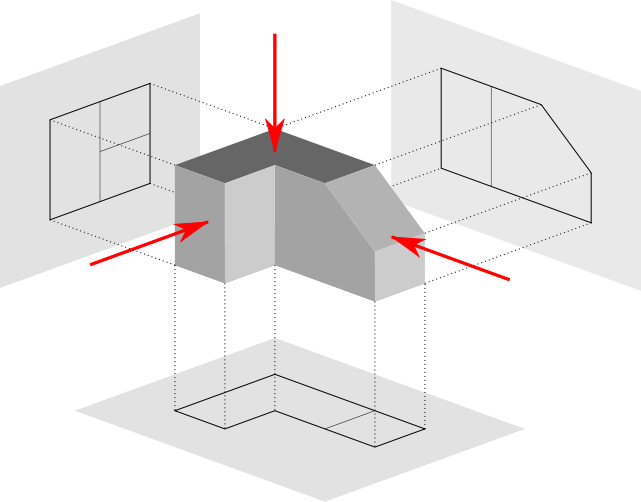
\includegraphics[scale=0.5]{imagini/proiectie/ortografica.png}
      \caption{Proiecția ortografică a unui corp \protect\footnotemark}
      \label{fig:proj}
  \end{center}    
\end{figure}

\footnotetext{\url{https://www.kisspng.com/png-graphical-projection-orthographic-projection-multi-1362397/download-png.html}}

O proiecte ortografica simpla, pe planul \(z=0\) poate fi definita de urmatoarea matrice:

\[
P=
  \begin{bmatrix}
    1 & 0 & 0 \\
    0 & 1 & 0 \\
    0 & 0 & 0 
  \end{bmatrix}
\]

Pentru fiecare punct \(v=(v_x,v_y,v_z)\), punctul transformat ar fi:

\[
P_v=
  \begin{bmatrix}
    1 & 0 & 0 \\
    0 & 1 & 0 \\
    0 & 0 & 0 
  \end{bmatrix}
  \begin{bmatrix}
    v_x  \\
    v_y  \\
    v_z  
  \end{bmatrix}
  =
  \begin{bmatrix}
    v_x  \\
    v_y  \\
    0  
  \end{bmatrix}
\]

\subsection{Aplicare}

Acest concept a fost aplicat pentru reprezentarea elementelor care formeaza intregrul model 3D. 
Setul de date nu contine dimensiunile exacte ale elementelor ci doar punctele de legare cu late elemente si centrul de greutate.
Prin calcularea punctelor simetrice ale punctelor de legare la centrul de greutate și prin incadrarea unui dreptunghi in jurul lor
obtinem forma care v-a reprezenta elementul in sine.\newline 

Aplicația conține trei moduri de afișare a modelului, fiecare perspectivă folosind coordonatele \((x,y,z)\) din setul de date 
eliminand una din ele pentru reprezentarea in 2D:
\begin{itemize}
\item Perspectva de deasupra, folosind \((x,y)\)     
\item Perspectva laterală, folosind \((x,z)\)
\item Perspectva frontala, folsind \((y,z)\)
\end{itemize}
\newpage
\section{Tehnologii folosite}
\subsection{C++}

C++ este un limbaj de programare creat de Bjarne Stroustrup ca o extensie a limbajului C, inițial fiind numit "C cu clase". 
Limbajul s-a extins semnificativ, C++ modern având caracteristici orientate pe obiect, de programare generica și funcțională 
precum și accesul la manipularea memoriei. Este aproape întotdeauna implementat ca limbaj compilat, iar mulți furnizori oferă 
compilatoare C ++, inclusiv LME, LLVM, Microsoft, Intel și IBM, astfel încât limbajul sa poată fi compilat pe mai multe platforme.\newline 

A fost conceput cu o înclinare către programarea sistemelor și programarea embeded, software limitat de resurse și sisteme mari, 
punând în prim plan performanta, eficienta și flexibilitatea ca și caracteristici esențiale ale limbajului. C++ s-a dovedit 
fiind util și în alte contexte precum aplicații desktop, servere, centrali telefonice.\newline

C ++ este standardizat de către Organizația Internațională pentru Standardizare (ISO), cu cea mai recentă versiune standard 
publicată de ISO în decembrie 2017 ca ISO / IEC 14882: 2017 (informal cunoscut sub numele de C ++ 17). Înainte de standardizarea 
inițială din 1998, C ++ a fost dezvoltat de omul de știință danez Bjarne Stroustrup la Bell Labs din 1979, ca extensie a 
limbajului C; el dorea un limbaj eficient și flexibil similar C, care să ofere și caracteristici de nivel înalt pentru organizarea 
programelor.\newline

\subsection{Qt}

Qt este un toolkit open-source și gratis folosit la crearea de interfețe grafice dar aplicații cross-platform care 
pot fi rulate pe diverse platforme hardware si software precum Linux, Windows, macOS, Adroid sau sisteme embeded, 
cu puține sau nici o schimbare in codul de baza dar păstrând funcționalitatile native. Qt este momentan dezvoltat 
de The Qt Company sub Qt Project prin guvernare open-source, în care sunt implicate mai multe organizații și dezvoltatori 
individuali cu scopul de aduce noi funcționalități Qt-ului.\newline

Majoritatea programelor GUI dezvoltate cu Qt au o interfață nativa similara cu cea a sistemului pe care este rulat. 
Aplicații precum unelte ce pot fi rulate din linia de comand sau console pentru servere, fără interfață grafica pot fi 
dezvoltate în Qt. Un exemplu fiind framework-ul web Cutelyst.\newline

Qt suporta diverse compilere ca GCC C++ și MSVC de la Visual Studio. Qt conține și Qt Quick, care include propriul 
limbaj de scriptare numit QML, care a facilitat dezvoltarea rapida a aplicațiilor mobile păstrând opțiunea de a scrie 
logica în C++ pentru cele mai bune rezultate în legătura cu performanta.\newline

Alte funcționalități includ acces la baze de date prin SQL, cititor de XML, cititor de JSON, managementul thread-urilor.\newline

Qt este construit pe aceste concepte:
\begin{itemize}
    \item Abstractizarea interfeței grafice
    
    La început Qt folosea propriul engine de desenare pentru a emula aspectul diferitelor platforme de pe care rula. 
    Astfel doar câteva clase depindeau de platforma făcând portarea mult mai ușoară, însa emularea nu era mereu perfecta. 
    Versiunile mai noi de Qt folosesc API-uri native de pe platforma de rulare, pentru a rezolva problemele din trecut.

    \item Signals si slots
    
    Este un concept introdus în Qt pentru comunicarea intre obiecte, având la baza conceptul șablonului de proiectare observer 
    evitând cod boilerplate. Obiectele ce țin GUI pot transmite semnale ce conțin informații relative la un eveniment care pot 
    fi captate de alte obiecte care conțin socluri.

    \item Compilator de metaobiecte

    Numit și moc, este o unealta care rulează pe codul unei aplicații Qt. Interpretează anumite macro-uri scrise în codul 
    sursa C++ și le folosește pentru a genera cod C++ cu ajutorul unor informații legate de clasele din aplicație. 
    Acest concept este folosit pentru a adăuga funcționalitati care nu sunt prezente nativ în limbajul C++: semnale și socluri, 
    introspecție, apelări asincrone de funcții.

    \item Legături intre limbaje

    Qt poate fi folosit și de alte limbaje precum Python, Javascript, C\# sau Rust.
\end{itemize}

\subsubsection{Graphics view framework}

Graphics View pune la disozitie un mediu în care se pot controla și se poate interacționa cu un număr mare de elemente grafice 2D. 
Framework-ul include și o arhitectura de propagarea a evenimentelor care facilitează interacțiunea cu elementele din scena. 
Elementele suporta evenimente legate de taste, mișcarea mouse-ul, evenimente de dublu click, etc. \newline

Graphics view folosește un arbore BSP (Binary Space Partitioning) care oferă o accesare rapida la oricare element, astfel se poate 
vizualiza și interacționa cu scene cu milioane de elemente grafice în timp real.\newline

Graphics view furnizează o abordare bazate pe elemente a programării model-view. Mai multe view-uri pot observa o scena, 
iar scena conține elementele grafice compuse dintr-o varietate de forme geometrice.\newline

\begin{itemize}
    \item Scena
    
    Clasa QGraphicsScene oferă următoarele funcționalități:
    \begin{itemize}
        \item O interfață pentru controlarea unui număr mare de elemente grafice.
        \item Propagarea evenimentelor din exterior către elemente.
        \item Setarea stării unui elemente, ex: selectie, focus.
    \end{itemize}

    Scena reprezinta un container pentru obiecte de tip QGraphicsScene. Elementele sunt adăugate prin funcția 
    \verb|QGraphicsScene::addItem()|, iar apoi pot fi accesate folosind una din multele funcții de returnare.Functia 
    QGraphicsScene::items() și supraincarcariile ei, returnează toate elementele grafice care se intersectează sau 
    care sunt conținute de un punct, un dreptunghi, un poligon sau un vector. QGraphicsScene::itemAt() returnează elementul 
    de la cel mai înalt nivel de suprapunere într-un anumit punct. Toate funcțiile returnează elementele într-o ordine 
    descendenta în legătura cu eventuale suprapuneri.\newline

    \begin{lstlisting}[language=C++]
        QGraphicsScene scene;
        QGraphicsRectItem *rect = scene.addRect(QRectF(0, 0, 100, 100));

        QGraphicsItem *item = scene.itemAt(50, 50);
    \end{lstlisting}

    Arhitectura de propagare a evenimentelor a clasei QGraphicsScene asigura transmiterea evenimentelor către 
    elemente dar și propagarea evenimentelor intre ele. Daca scene primește un eveniment legat de mouse la o anumita poziție, 
    scena transmite mai departe evenimentul către toate elementele care se afla în acel punct.\newline

    Scena totodată poate controla starea elementelor, de exemplu dacă elementele sunt selectate, sau sunt în focus relativ cu 
    evenimente de la tastatura. Mai multe elemente pot fi selectate folosind QGraphicsScene::setSelectionArea(). 
    Pentru a accesa toate elementele selectate se poate folosi QGraphicsScene::selectedItems(). O alta stare tratata este cea 
    de focus pe un anumit element. Se poate seta prin apelarea funcției QGraphicsScene::setFocusItem() sau QGraphicsItem::setFocus(), 
    iar pentru a accesa elementul curent în focus QGraphicsScene::focusItem().\newline

    \item View
    
    QGraphicsView furnizează un widget prin care se poate vizualiza conținutul unei scene. Se pot atasa mai multe view-uri la 
    aceeași scena dacă este nevoie. 

    \begin{lstlisting}[language=C++]
        QGraphicsScene scene;
        myPopulateScene(&scene);

        QGraphicsView view(&scene);
        view.show();

    \end{lstlisting}

    View-ul poate primii evenimente din exterior de la tastatura sau mouse și le trimite mai departe la scene 
    (făcând conversia la coordonatele scenei dacă este nevoie, deoarece în unele cazuri când scene este mai mare 
    decât fereastra view-ului, view-ul nu poate afișa toată scena, ci doar o porțiune).\newline
    
    Folosind matricea de transformare, QGraphicsView::transform(), view-ul poate scala sau rotii scena. 
    Pentru convenienta QGraphicsView oferă funcții pentru convertirea la, sau de la, coordonatele scenei la 
    coordonatele view-ului. QGraphicsView::mapToScene() si QGraphicsView::mapFromScene().\newline

    \item Elementul
    
    QGraphicsItem este clasa de baza pentru elementele grafice dintr-o scena. Graphics View oferă câteva elemente grafice 
    standard pentru forme simple, precum dreptunghi  (QGraphicsRectItem), elipsa (QGraphicsEllipseItem), dar și text 
    (QGraphicsTextItem). De obicei utilizatorul specializează clasa de baza prin moștenire pentru a obține elemente 
    grafice de forme diferite.\newline

    QGraphicsItem suporta următoarele functionalitati:
    \begin{itemize}
        \item evenimente de mouse (click, hover, scroll-wheel, etc.)
        \item evenimente de tastatura
        \item evenimente meniu de context
        \item grupare, fie prin relație părinte-copil, fie prin clasa QGraphicsItemGroup
        \item detecție de coliziuni
    \end{itemize}

    Toate elementele se afla într-un sistem de coordonate local, și la fel ca QGraphicsView, conțin funcții pentru 
    convertirea la coordonatele scenei. Totodată la fel ca și QGraphicsView sistemul de coordonate poate fi transformat 
    folosind o matrice,  QGraphicsItem::transform(). Acest lucru este folositor la scalarea sau rotirea individuala.\newline

    Elementele pot conține si alte element (copii). Transformările părintelui sunt moștenite de toți copiii.\newline
    
    QGraphicsItem suporta și detecție de coliziuni, prin funcțiile QGraphicsItem::shape() și QGraphicsItem::collidesWith(), 
    ambele funcții virtuale care pot fi suprascrise.\newline
\end{itemize}

\subsection{Aplicare}

Majoritatea acestor noțiuni au fost folosite la dezvoltarea aplicație. 
Fiecare tab deschis conține un QGraphicsView cu o scena cu toate elementele. 
View-ul este dinamic iar utilizatorul poate interacționa cu el, prin zoom sau prin schimbarea întregii scene, 
selectând diferite perspective. Fiecare element grafic din aplicație, moștenește clasa de baza QGraphicsItem, 
fiind specializat pentru diferitele tipuri care trebuie afișate. De exemplu obiectele de tip Motion body sunt 
afișate ca dreptunghiuri albastre de diferite forme în funcție de datele din fișierul sursa. Aceste elemente 
pot fi mutate cu mouse-ul. Elementele de tip Motion body pot fi conectate de alte elemente Motion body fie prin 
printr-un Joint sau Connector. La fel pentru Joint și Connector s-au folosit implementări separate pentru afișarea 
diferitelor tipuri. Utilizatorul poate interacționa cu toate elementele prin click-dreapta pentru a deschide un meniu de context. 
Prin acest meniu el poate schimba culoarea, reseta culoarea sau deschide un panou în care sunt afișate informații adiționale 
elementului.\newline







\newpage
\section{Grafica turtle}

Este o modalitate de desenare care se bazează pe câteva rutine simple. Ne putem imagina ca fiind un cursor care desenează 
linii drepte într-un plan cartezian. Cursorul are trei atribute: o locație, o orientare (sau o direcție) și un pix. 
Pixul are de asemenea, atribute: culoare, lățime și stare(desenare / inchis).\newline

Cursorul se muta cu comenzi care sunt relative la poziția sa, cum ar fi "înainte 10 pixeli" și "rotiți cu 90 de grade". 
Pixul purtat de cursor poate fi de asemenea controlat, având posibilitatea de a îi schimba culoarea sau lățimea.\newline

Un sistem complet de grafica necesita un flux de control, proceduri si recursivitate. Din aceste metode se pot construi forme mai complexe, cum ar fi pătrate, triunghiuri, cercuri și alte figuri compuse. 
Ideea de grafica turtle, de exemplu, este utilă într-un sistem Lindenmayer pentru generarea de fractali.\newline

Geometria graficii turtle funcționează oarecum diferit față de geometria carteziană, 
fiind bazată în primul rând pe noțiunea de vector (direcția relativă și distanța față de punctul de pornire). \cite{turtle2}\newline

\subsection{Aplicare}

\lstset{language=C++}
\begin{lstlisting}
    class Turtle
    {
    public:
        Turtle(double x, double y, double dir);
        void rotate(double angle);
        void forward(double length, bool draw = true);
        Path getPath()const;
    private:
        double x,y,dir;
        Path path;
    };
\end{lstlisting}

De exemplu pentru a desena un triunghi echilateral cu lungimea laturilor de 100 de unități.\cite{turtle}

\lstset{language=C++}
\begin{lstlisting}
    forward(100);
    rotate(PI/3);
    forward(100);
    rotate(PI/3);
    forward(100)
\end{lstlisting}

Fiecare comanda schimba starea Turtle-ului si a traseului desenat. 
Cele trei comenzi de forward desenează laturile triunghiului de lungime \(100\), adăugând latura la traseul total parcurs. 
Comenzile de \verb|rotate| schimba direcția de desenare cu \(60\)\degree \footnote{in exemplul pentru desenare am folosit \(PI\) ca reprezentand \(180\)\degree, astfel \(180\degree \div 3 = 60\degree\)}. 
După ultima comandă de forward pixul se afla în punctul inițial de desenare, dar datorita lipsei unei comenzi \verb|rotate| de \(60\)\degree, 
direcția de desenare este diferită de cea inițiala.\newline

Folosind structuri repetitive putem abstractiza metoda de desenare. De exemplu pentru desenarea unui poligon regulat convex\cite{turtle}:

\begin{lstlisting}
    polygon(nrOfEdges){
    for(i=1;i<nrOfEdges;i++):
        forward(2*PI/nrOfEdges);
        rotate(2*PI/nrOfEdges);	
    }
\end{lstlisting}

Pentru \verb|nrOfEdges=3| avem din nou un triunghi echilateral, pentru \verb|nrOfEdges=4| avem un pătrat, și asa mai departe. 
Folosind un \verb|nrOfEdges| destul de mare, lungimea laturii scade si putem ajunge la o forma care într-un spațiu discret 
este similara cu un cerc.\newline 

\begin{figure}[H]
    \begin{center}
        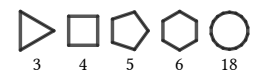
\includegraphics[scale=1]{imagini/turtle/circle.png}
        \caption{Desenarea unei forme similare cu un cerc \protect\footnotemark}
        \label{fig:tabs}
    \end{center}    
\end{figure}

\footnotetext{imagine preluata din \cite{turtle}}

Extinzând aceste metode elementare de desenare putem ajunge la modalități de desenare pentru simboluri mai complexe 
formate din forme geometrice simple. (ex desenarea proiecției unui cilindru într-un plan 2D, anexa 12.2). \newline

\begin{figure}[H]
    \centering
    \subfloat[Joints]{{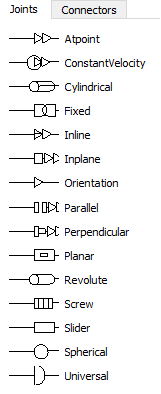
\includegraphics[scale=0.8]{imagini/turtle/joints.png} }}%
    \qquad
    \subfloat[Connectors]{{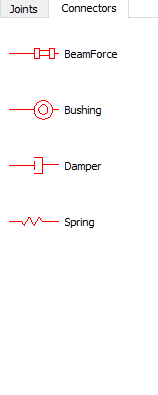
\includegraphics[scale=0.8]{imagini/turtle/connectors.png} }}%
    \caption{Simbolurile desenate prin turtle graphics pentru fiecare tip de connector sau joint}%
    \label{fig:example}%
\end{figure}


Pentru implementarea mea a acestui concept am adaugat funcțiile \verb|save()| și \verb|load()| pentru a eficientiza procesul de desenare.
Funcția \verb|save()| salvează starea curentă a clasei, și anume coordonatele x,y și direcția în acel moment. Astfel dacă vrem să ne întoarcem 
într-un punct precedent nu mai este nevoie sa facem pașii necesari sa ne întoarcem in acel punct, ci putem apela direct funcția \verb|load()|.\newline

\newpage

Secvența de cod corespunzatoare implementării structurii de stare:

\lstset{language=C++}
\begin{lstlisting}
struct State
{
    State(double x, double y, double dir) 
    double m_x;
    double m_y;
    double m_dir;
};
\end{lstlisting}

Clasa adaptată:

\lstset{language=C++}
\begin{lstlisting}
class Turtle
{
public:
    Turtle(double x, double y, double dir);
    Turtle(QPointF start, double dir);
    void rotate(double angle);
    void forward(double length, bool draw = true);

    void save();
    void load();

    QPainterPath getPath()const;
private:
    QPainterPath m_path;
    State m_current;
    State m_saved;
};
\end{lstlisting}



\newpage
\section{XML}

Extensible Markup Language (XML) este un meta-limbaj de marcare care definește un set de reguli de scriere astfel în cat sa poată fi citit și de oameni dar și de calculator într-un mod eficient. X-ul din XML vine de la eXtensibil, ceea ce înseamnă ca acest limbaj poate fi adaptat și proiectat în funcție de nevoia utilizatorului. Trebuie remarcat faptul ca, în ciuda numelui sau XML în sine nu este un limbaj de marcare, este un set de reguli prin care utilizatorul își poate dezvolta propriul limbaj.

XML este un standard aprobat de W3C pentru documentele de marcare. Acesta oferă o
sintaxa generică folosită pentru a marca date din document cu tag-uri, într-un mod flexibil care poate fi adaptat pentru a satisface anumite cerințe din domeniul în care este aplicat.

\subsection{Aspecte}

\begin{enumerate}[wide=0pt, listparindent=1.25em, parsep=0pt]
\item Descriptiv

XML oferă utilizatorilor libertatea de a-și crea propriul limbaj de marcare pentru un scop specific.
Astfel se pot crea un număr nelimitat de limbaje pentru a satisface o anumita necesitate.

\item Meta-date

Meta-datele se refera la “date care descriu date”. 
Acest lucru este esențial deoarece degeaba avem date dacă nu știm cum sa le interpretam. 
XML are o metoda standard și sintaxa pentru a expune atât datele cat și meta-datele. 
De exemplu  pentru <country>Romania</country>, “country” reprezinta mete-data, iar “Romania” este data în sine. 
Astfel putem aveam mai multe date atribuite aceleiași meta-date: 
\newline<country>Romania</country>
\newline<country>France</country>

\item Portabilitate

XML oferă potențialul de partajare a datelor pe diferite platforme. 
Scopul de baza din spatele XML este scrierea documentelor într-un mod care poate fi transmis de la un mediu la altul păstrând 
integritatea datelor. Acest lucru este facilitat prin faptul ca documentele XML sunt text și astfel orice instrument ce poate 
citi un document text poate interpreta un document XML. 

\item Structura neambigua

Chiar dacă XML este flexibil în definirea elementelor este strict în alte aspecte, 
iar utilizatorii trebuie sa urmeze un set de reguli predefinite. 
Aceste reguli restricționează modul în care un document este scris astfel încât sa nu exista ambiguitate în interpretarea numelor, 
ordinii elementelor sau ierarhiei de elemente. Astfel se minimizează eventuale erori ce pot apărea și complexitatea textului, 
iar parser-i de XML pot interpreta datele cu ușurința fără apariția de erori pe parcurs.\newline 

Utilizatorii sunt, de asemenea, liberi să creeze reguli privind modul în care ar trebui să arate documentele.
Definirea tipului de document (DTD) și schemele XML sunt instrumentele care ajută la acest
proces.
\end{enumerate}

\subsection{Terminologie}

\begin{enumerate}[wide=0pt, listparindent=1.25em, parsep=0pt]
    \item Caracter - un document XML este format din string-urui de caractere. Aproape orice caracter unicode poate apărea într-un document.
    \item Marcaj - documentul este împărțit în marcaje și conținut care pot fi observate după reguli sintactice. In general textul care formează în marcaj începe cu caracterul "<" și se termina cu ">". 
    \item Tag - reprezinta un marcaj si poate fi :
    \begin{itemize}
        \item de inceput : <sectiune>
        \item de sfarsit : </sectiune>
        \item fara continut : <line-break/> 
    \end{itemize}
    \item Element - este o componenta a documentului care începe cu un tag de început și se termina cu un tag de 
    sfârșit corespunzător. Datele intre tag-uri constituie conținutul elementul care poate cuprinde și alte elemente.\newline 
    ex:<greeting>Hello, world!</greeting>
    \item Atribut - un atribut consta într-o pereche de tip nume-valoare care se poate afla într-un tag de început sau 
    într-un tag fără conținut.\newline 
    Un exemplu este <img src = "imagine.jpg"/>, unde numele atributului este "src" iar valoare 
    este "imagine.jpg". Un atribut poate avea o singura valoare și poate apărea cel mult o data în tag-ul unui element. 
    \item XML prolog - Un prolog este linia inițiala într-un document XML. Conține de obicei versiunea de XML și tipul de encoding.\newline 
    De exemplu: <?xml version="1.0" encoding="UTF-8">
    \item Arborele XML Structura unui document XML poate fi considera ca fiind un arbore. 
    Documentul începe cu o rădăcina și se ramifica în mai multe frunze. 
    Elementul rădăcina conține toate elementele documentului și nu are părinte, ca restul elementelor.
\end{enumerate} 

\subsection{Aplicare}
Aplicația lucrează cu trei tipuri de elemente: Motion body, Joint, Connector. 
Motion body-urile sunt obiecte care sunt conectate intre ele fie cu joint-uri fie cu connector-i. 
Joint reprezinta un punct fix intre doi motion body, iar connector este o legătura.(?)

\newpage
\section{Simcenter}

CAE(Computer-aided engineering) este un termen care definește un tip de aplicație folosit în domeniul ingineriei. Aceste aplicații sunt folosite pentru
 a rezolva diferite probleme ce țin de arii științifice precum: analiza finită a elementelor (FEA), mecanica fluidelor numerică (CFD), 
 durabilitatea materialelor și optimizare. Acest tip de aplicație este folosit pentru a analiza rezistența și performanța anumitor componente 
 sau ansambluri de componente, eficientizând timpul și materia necesara în întregul proces, in special datorita aspectului digital.
Este folosit în multe domenii precum industria de auto-motive, aviație și aeronautica. \cite{cae}\newline

Ariile acoperite de CAE sunt:
\begin{itemize}
\item analiza stresului anumitor componente folosind FEA
\item analiza fluidelor prin CFD
\item cinematica
\item simularea formării unei componente prin turnarea sau presarea materialelor de construcție
\item optimizarea produsului 
\item optimizarea procesului de creare
\end{itemize}

In general sunt trei etape care formează întregul proces de analiza:
\begin{itemize}
    \item pre-procesare: se definește modelul și factorii de mediu 
    \item analiza: proces care este rulat pe o unitate de calculare performanta
    \item post-procesarea: se afișează rezultatele utilizând aplicații de vizualizare
\end{itemize}

Acest ciclu este rulat iterativ de mai multe ori fie manual fie prin aplicații de optimizare.\newline

Aplicațiile CAE sunt folosite foarte des în industria de automotive. Folosirea lor a dat posibilitatea de a 
reduce costul și timpul de producție în timp ce au îmbunătățit siguranța, confortul și durabilitatea vehiculelor produse. 
S-a ajuns în punctul în care se preferă testarea produselor într-un mediu digital decât pe un prototip fizic.\cite{cae}\newline

Simcenter Motion este o aplicație software CAE folosită pentru animarea și analizarea mecanismelor cinematice și dinamice în 
legătură cu puncte de design critice, forțe, viteze, accelerații. \cite{cae2}\newline

Într-o simulare cinematică:
\begin{itemize}
    \item sarcinile externe și forțele de inerție afectează forțele de reacție ale corpurilor dar nu afectează mișcarea
    \item corpurile și legăturile dintre ele sunt rigide
    \item nu există bucșe sau alte elemente care se pot deforma
\end{itemize}

\begin{figure}[H]
    \begin{center}
        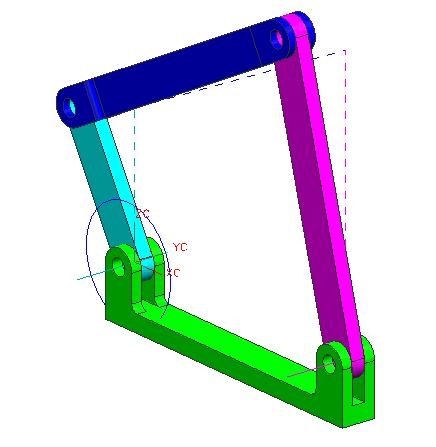
\includegraphics[scale=0.7]{imagini/simcenter/cinematica.png}
        \caption{Model cinematic \protect\footnotemark}
        \label{fig:cinematic}
    \end{center}    
\end{figure}

\footnotetext{imagine preluată din \cite{cae2}}

\newpage

Într-o simulare dinamică:
\begin{itemize}
    \item sarcinile externe și forțele pot genera mișcare
    \item există bucșe pentru simularea legăturilor de supunere
    \item există efecte ce țin de forțe de frecare și contact 
    \item se poate rula o analiză de echilibru static în care toate forțele externe și interne sunt în echilibru
\end{itemize}

\begin{figure}[H]
    \begin{center}
        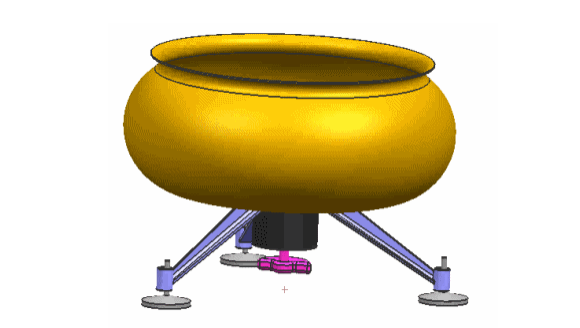
\includegraphics[scale=0.7]{imagini/simcenter/dinamic.png}
        \caption{Model dinamic \protect\footnotemark}
        \label{fig:dinamic}
    \end{center}    
\end{figure}

\footnotetext{imagine preluată din \cite{cae2}}

In aplicație un mecanism se definește ca fiind un ansamblu de componente rigide care se mișcă coeziv. 
Pentru a crea un mecanism este necesară:
\begin{itemize}
    \item specificarea corpurilor de mișcare și a corpurilor statice
    \item constrângerea mișcării dintre corpuri, prin definirea mișcării unui corp în legătură cu celelalte corpuri. 
    Acestea se crează prin legături dintre corpurile de mișcare.
    \item setarea întregii mișcări ale mecanismului
\end{itemize}

\begin{figure}[H]
    \begin{center}
        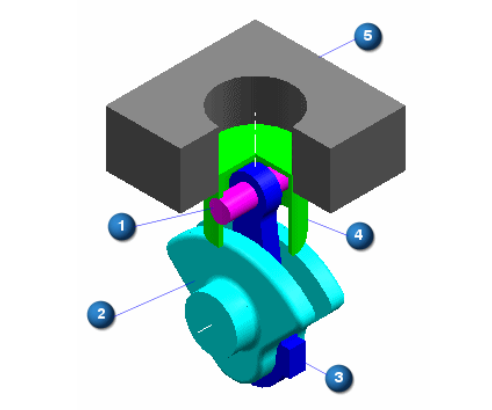
\includegraphics[scale=0.7]{imagini/simcenter/mecanism.png}
        \caption{Model mecanism \protect\footnotemark}
        \label{fig:mecanism_simplu}
    \end{center}    
\end{figure}

\footnotetext{imagine preluată din \cite{cae2}}

Corpurile de mișcare reprezintă elemente rigide în mecanism. Orice componentă din model ce se poate mișca trebuie 
înclusa într-un corp de mișcare. Un corp de mișcare poate fi reprezentat fie printr-o componentă de asamblare fie 
prin corpuri geometrice simple solide, linii curbe sau puncte. De obicei este mai ușor în procesul de creare a mecanismului să 
fie definit inițial prin elemente simple precum linii curbe și puncte pentru a verifica un comportament elementar 
ca apoi detaliile sa fie adăugate.\newline

\begin{figure}[H]
    \begin{center}
        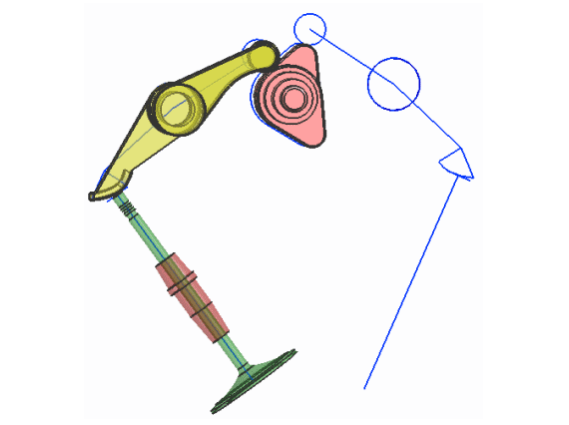
\includegraphics[scale=0.7]{imagini/simcenter/body.png}
        \caption{Model mecanism format din forme simple\protect\footnotemark}
        \label{fig:mecanims_curbe}
    \end{center}    
\end{figure}

\footnotetext{imagine preluată din \cite{cae2}}

Într-un mecanism un grad de libertate descrie cum un corp de mișcare se poate deplasa relativ la celelalte corpuri. 
Toate gradele de libertate ale unui mecanism descriu toate mișcările independente posibile ale lui. Fară constrângeri 
un corp dintr-un mecanism plutește în spațiu avand șase grade libertate: trei grade de translație (direcția X, Y sau Z) 
și trei grade de rotație (în jurul axelor X, Y sau Z). O îmbinare ale corpurilor constrânge unu sau mai multe grade libertate. \cite{cae2}\newline

Mișcarea unui corp este definită ca fiind mișcarea lui relativa la un corp de baza de care este legat, sau la pământ dacă nu exista.\newline

Aplicația creată are rolul de vizualiza relațiile dintre elementele prezente in model, ținănd cont de tipul lor și de tipul de legătura dintre ele.

\newpage
\section{Functionalități}

În acest capitol sunt prezentate funcționalitățile implementate în aplicația dezvoltată. Aplicația afișează o diagramă 
care are la baza un model 3D format din mai multe elemente, punând accentul pe relațiile de legătura dintre elemente.\newline

Funcționalități de bază:
\begin{itemize}
    \item încărcarea oricărui fișier .mdef și crearea diagramei
    \item modificarea diagramei create
    \begin{itemize}
        \item mutarea elementelor
        \item scalarea întregii diagrame
        \item schimbarea culorii anumitor elemente
    \end{itemize} 
    \item salvarea modificărilor într-un fisier separat
    \item încărcarea automată a fișierului salvat, dacă există
    \item afișarea modelului din mai multe perspective ortografice
    \item afișarea modelului sub formă de graf
    \item căutarea unui element dupa un cuvânt cheie și evidențierea lui
    \item compararea dintre diferite versiuni de modele
    \item afișarea unui panou de tip legendă care prezintă diferitele tipuri de elemente
    \item afișarea unui panou de informații în care sunt afișate informații adiționale legate de elementele selectate
\end{itemize}

În continuare sunt prezentate caracteristicile aplicației în detaliu. Pentru demonstrarea funcționalităților am folosit un fișier .mdef
pe baza modelului urmator. Modelul a fost ales datorita structurii simetrice și a tipurilor diferite de legături din model.

\begin{figure}[H]
    \begin{center}
        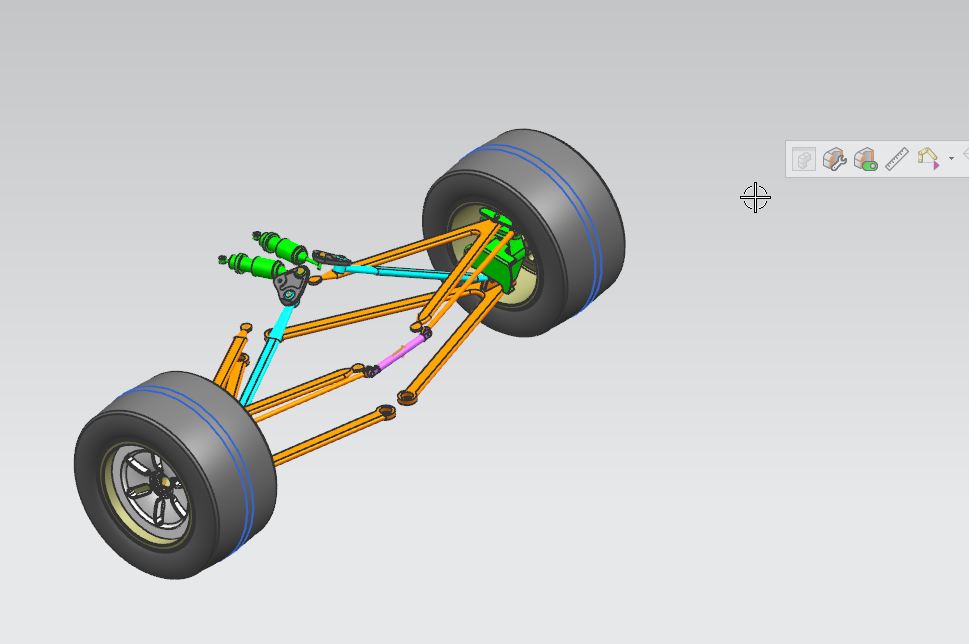
\includegraphics[scale=0.3]{imagini/implementare/model.png}        
    \end{center}
    \caption{Porțiunea de suspensii de la o mașină}
    \label{fig:tabs}
\end{figure}

\subsection{Încarcarea fișierelor}
Se pot încărca oricâte fișiere .mdef în aplicație, fiecare fișier fiind deschis într-un tab diferit. 
Acest lucru se face din meniul \verb|File| de unde se alege opțiunea \verb|Open|, care v-a deschide o nouă fereastră de 
unde utilizatorul își poate alege fișierul. 
Odată ales un fișier el este deschis într-un tab nou care conține o scenă cu mai multe elemente de tip Motion body, 
Joint sau Connector.\newline

\begin{figure}[H]
    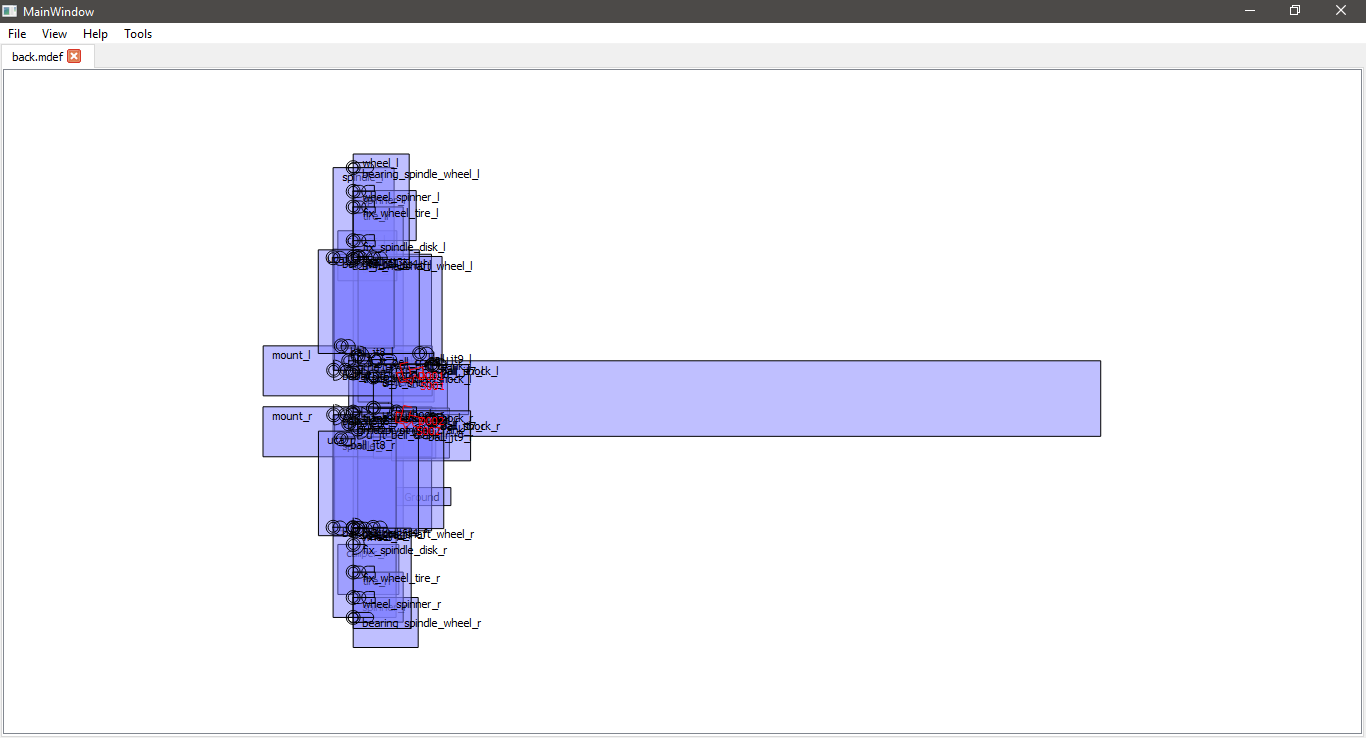
\includegraphics[width=\linewidth]{imagini/implementare/overlapping.png}
    \caption{Modelul menționat anterior deschis în aplicație}
    \label{fig:tabs}
\end{figure}

\subsection{Modificarea diagramei}
Diagrama creată se poate modifica prin:
\begin{itemize}
    \item schimbarea perspectivei ortografice
    \item afișarea sub formă de graf
    \item scalare
    \item modificarea pozițiilor elementelor
    \item modificarea culorii elementelor
\end{itemize}

Una dintre problemele întâmpinate în procesul de dezvolatere a aplicației a fost suprapunerea elementelor în anumite perspective. 
Această problemă a fost rezolvată prin două metode: prin scalare, care păstreaza pozițiile relative ale elemntelor în model, și prin afișarea 
modelului sub forma unui graf, care nu ia în considerare aspecte legate de poziții sau forme.\newline


Scalarea este necesară pentru modele mari având scopul de a pune în evidență detalii care s-ar observa greu dacă întregul model este afișat în fereastră. 
Totodată pentru modul de afișare sub forma unei perspective ortografice, scalarea este utilă
pentru modelele în care se suprapun elemente. În acel mod prin scalare se scalează doar punctele de conectare ale legaturilor cu corpurile, în schimb ce marimea 
corpurilor ramâne la fel.\newline

\begin{figure}[H]
    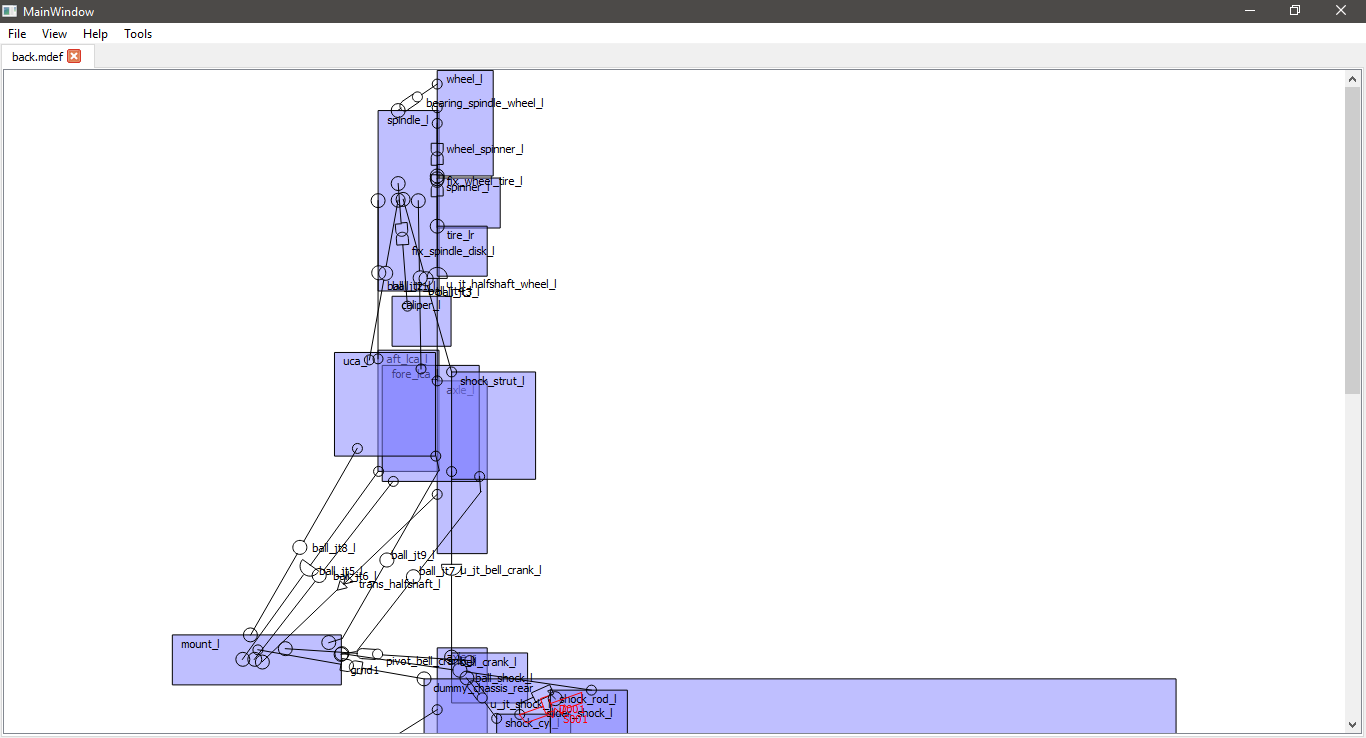
\includegraphics[width=\linewidth]{imagini/implementare/overlappingzoom.png}
    \caption{Modelul menționat anterior scalat}
    \label{fig:tabs}
\end{figure}

Mutarea elementelor poate fi utilă în cazul în care utilizatorul vrea să organizeze în alt fel reprezentarea fișierul, sau daca există
anumite suprapuneri între elemente.\newline 

\subsection{Salvarea scenei modificate}
Toate schimbările legate de scena în care se află toate elementele pot fi salvate într-un fișier XML separat. 
Dacă un model are salvată o scenă, ea este încărcată automat la deschiderea modelului.
Pentru salvarea automată se alege opținuea \verb|Save| din meniul \verb|File|, fișierul salvat se v-a afla într-un folder specific și v-a avea acelasi nume cu modelul.
Dacă se dorește ca modelul să fie salvat explicit într-un loc anume cu un nume diferit se poate alege \verb|Save as|. La fel dacă se dorește 
încărcarea unui fișier salvat anume, se elege opțiunea \verb|Load file|.

\subsection{Afișarea sub forma unei perspective ortografice}
Fișierul reprezentând un model 3D, pentru a afișa structura de bază și relațiile dintre elemente în sine într-un plan 2D am 
ales folosirea noțiunii de perspective ortografice. Modelul este desenat în 2D, avand la bază coordonatele modelului
3D din fisierul .mdef, pentru fiecare perspectivă folosindu-se doua dintre cele trei coordonate.
Astfel se obțin trei perspective individuale pentru afișarea modelului:

\begin{itemize}
    \item perspectiva laterala (side)
    \item perspectiva frontala (front)
    \item perspectiva de deasupra (top)
\end{itemize} 


\begin{figure}[H]
    \begin{center}
    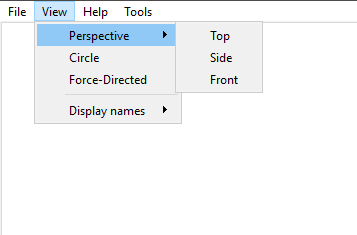
\includegraphics[scale=0.7]{imagini/implementare/viewmenu.png}
    \end{center}
    \caption{Meniul view}
    \label{fig:tabs}
\end{figure}

Când un model este încărcat el este deschis automat în perspectiva laterală.
Formele elementelor din această opțiune au la bază coordonate reale citite din fișier. De exemplu mărimea dreptunghiului 
care reprezintă un Motionbody este calculată în funcție de pozițiile conexiunilor cu alte elemente și centrul de 
greutate. Aceste perspective pot fi alese de utilizator selectănd \verb|Perspective| din meniul \verb|View|. \newline

Această abordare este folositoare, din perspectiva utilizatorului, doar pentru modele cu un număr mic spre mediu de elemente 
deoarece pentru modele mai mari s-a observat că datorită structurii lor, în multe cazuri existau suprapuneri în oricare dintre 
cele trei perspective, făcând înțelegerea modelului mult mai grea.\newline 


\subsection{Afișarea sub formă de graf}
Pentru cazuri în care apar multe suprapuneri s-a implementat o structura de graf pentru reprezentarea modelului. 
În comparație cu perspectiva ortografică nu se ține cont de date precum puncte de conexiune sau centru de greutate și se bazează 
strict pe relațiile dintre elemente. Folosind un algoritm force-directed de desenare a unui graf obținem o structură mult mai organizată 
și mai inteligibilă, însa renunțam la concepte legate de forma modelului sau pozițiile elementelor în model.\newline
 
\begin{figure}[H]
    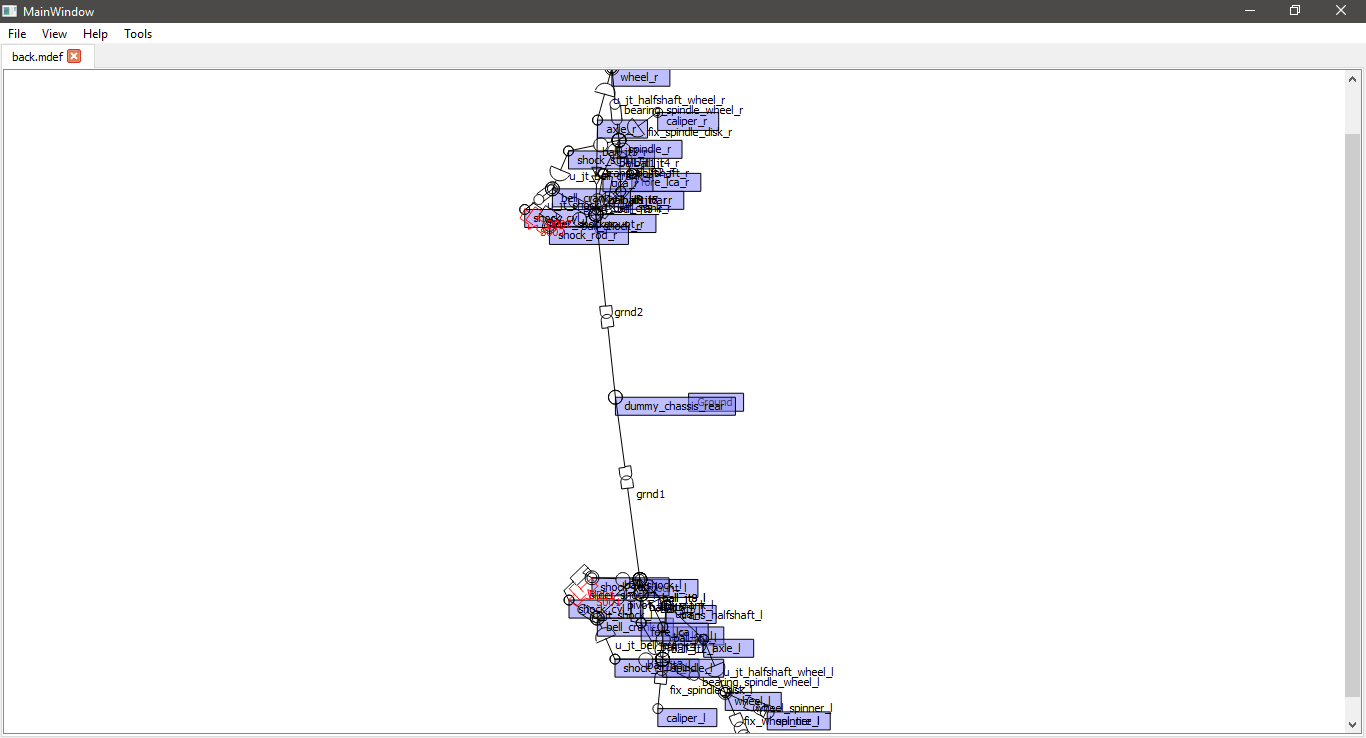
\includegraphics[width=\linewidth]{imagini/implementare/graf.png}
    \caption{Modelul menționat sub structura de graf}
    \label{fig:tabs}
\end{figure}

\begin{figure}[H]
    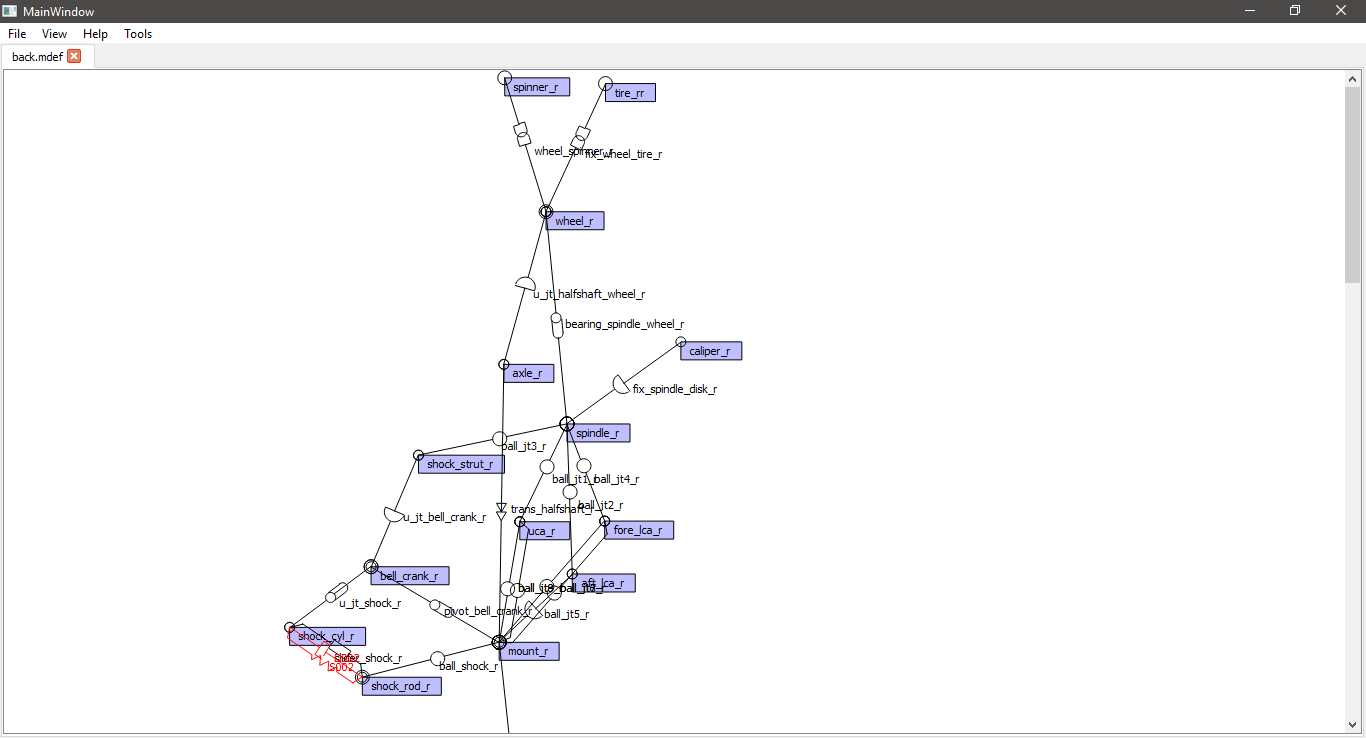
\includegraphics[width=\linewidth]{imagini/implementare/grafzoom.png}
    \caption{Același graf scalat}
    \label{fig:tabs}
\end{figure}

Această funcționalitate a fost adăugată având în gând un concept prezent în algoritmii force-directed și anume cel care garantează ca dacă un graf este planar, desenarea 
lui nu va conține suprapuneri între muchii, și cel mai important, între noduri. Totodata și pentru grafuri care nu sunt planare desenarea 
lui conține un număr minim de suprapuneri între muchii, de multe ori neglijabil, modelul fiind în continuare ușor de înțeles.\newline

Opțiunea de graf poate fi aleasă alegând \verb|Force-directed| din meniul \verb|View|. În această perspectivă se pot evidenția și tipurile de elemente Joint mai bine deoarece nu mai 
sunt reprezentate ca un punct fix dintre doua elemente Motion body ci dintr-o muchie cu un simbol pentru tipul elementului. 
Totodată din meniul de view se poate alege dacă este necesară afișarea fiecărui nume ale elementelor, acest lucru se face din meniul \verb|View| alegând \verb|Show names|, 
de unde se poate deselecta câte o căsuță pentru fiecare tip de element.\newline 


\subsection{Căutarea elementelor}
În continuare, pentru înțelegerea mai buna a modelului au fost implementate niște funcționalități de ajutor. 
O funcție de căutare pune în evidență anumite elemente din model. Se poate accesa din meniul \verb|Tools| de unde este deschisa o nouă fereastră cu mai multe opțiuni de cautare. 
Căutarea după un sub-string al cuvântului cheie sau căutarea după întreg cuvântul. Este prezentă și o opțiune de regex prin care utilizatorul poate 
cauta elemente după un anumit șablon. Din aceeași fereastra se poate alege dacă vrem sa cautam doar după anumite tipuri 
de elemente, precum și culoarea de selectare. După ce apăsam search, dacă căutarea a avut succes elementele sunt evidențiate în scena cu o culoare aleasă.
Utilizatorul poate efectua mai multe căutari cu diferite culori, lucru folositor pentru organizarea elementelor. 

\begin{figure}[H]
    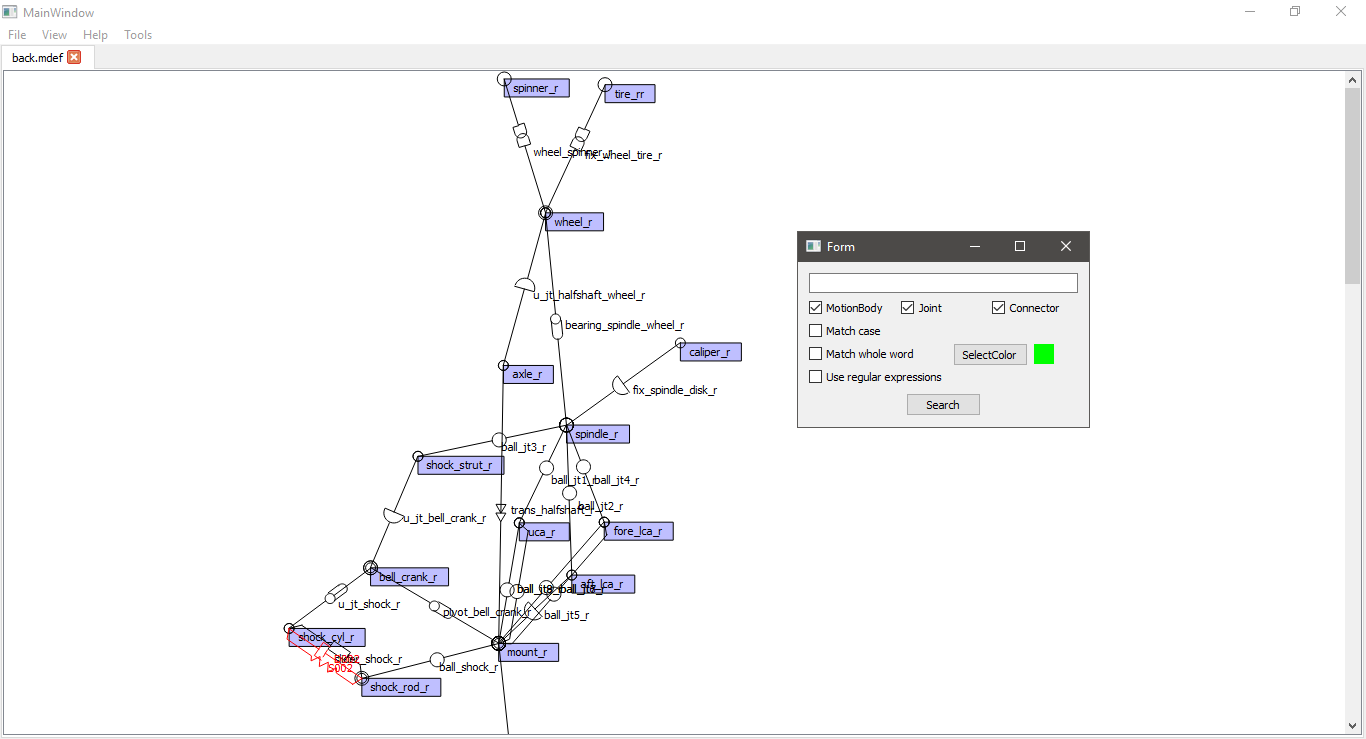
\includegraphics[width=\linewidth]{imagini/implementare/searchwindow.png}
    \caption{Fereastra de cautare}
    \label{fig:tabs}
\end{figure}

\begin{figure}[H]
    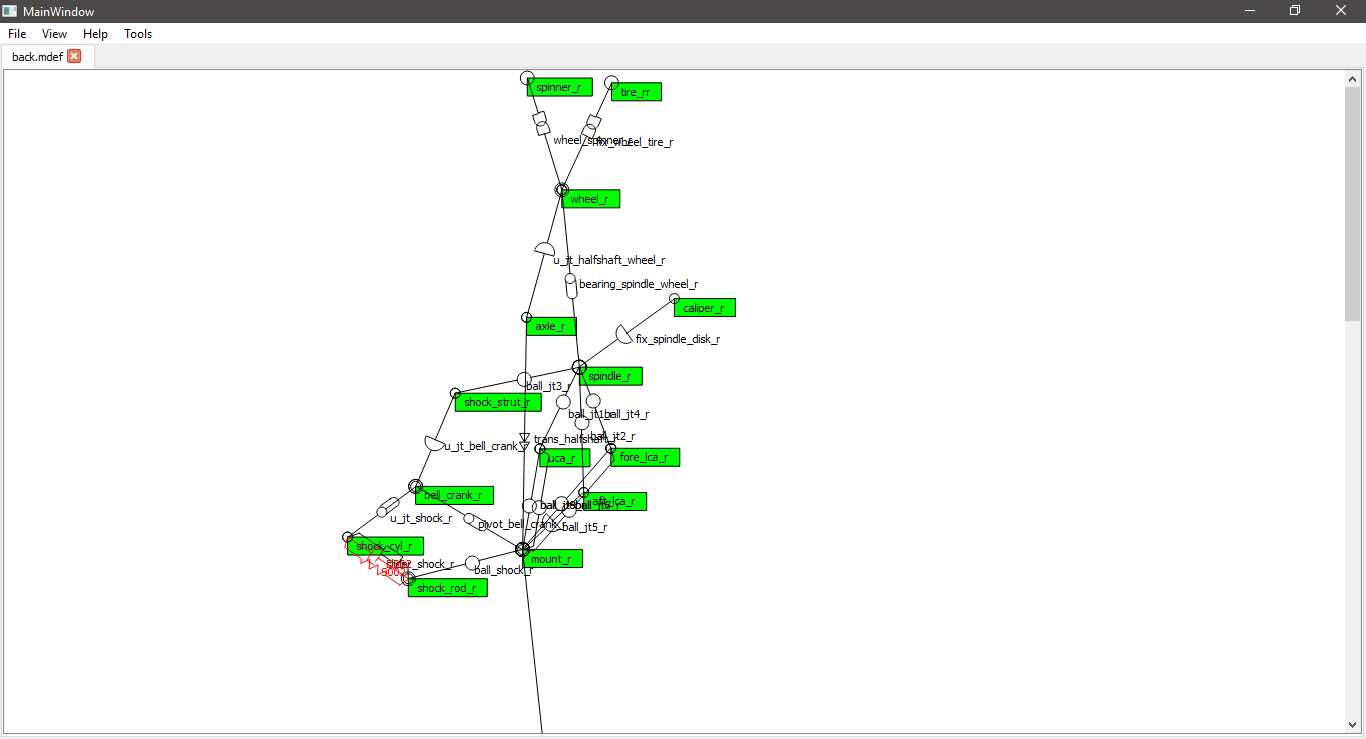
\includegraphics[width=\linewidth]{imagini/implementare/searchscene.png}
    \caption{Elementele care se afla pe partea dreapta a modeluilui, evidențiate prin funcția de căutare}
    \label{fig:tabs}
\end{figure}

\subsection{Compararea modelelor}
Pentru evidențierea diferențelor dintre versiuni diferite de 
fișiere .mdef a fost implementată funcționalitatea \verb|Compare models|. Se poate accesa din meniul \verb|Tools|, opțiunea \verb|Compare models| și va deschide 
o nouă fereastră de unde utilizatorul poate alege ce modele vrea sa compare dintre cele deschise. Diferențe precum date diferite sunt evidențiate cu galben,
iar lipsa de elemente este evidențiată prin colorarea rosu, în modelul care conține elementul lipsă din modelul de comparare.\newline 

\begin{figure}[H]
    \begin{center}
    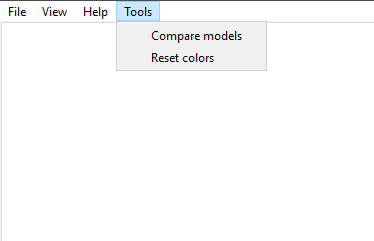
\includegraphics[scale=0.5]{imagini/implementare/toolsmenu.png}
    \end{center}
    \caption{Meniul Tools}
    \label{fig:tabs}
\end{figure}

\begin{figure}[H]
    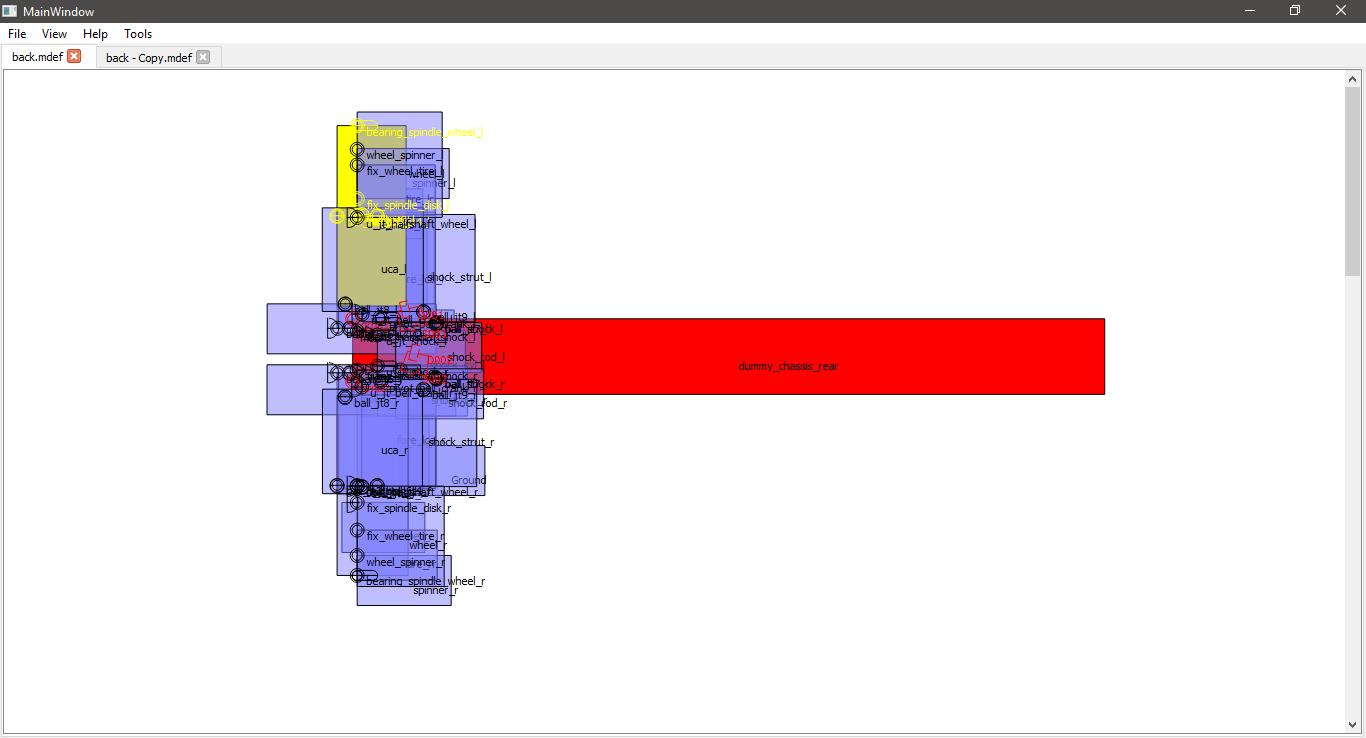
\includegraphics[width=\linewidth]{imagini/implementare/compare.png}
    \caption{Modelul principal comparat cu o alta versiune}
    \label{fig:tabs}
\end{figure}

\subsection{Informații adiționale}
O altă funcționalitate este cea a panoului de informații adiționale, acolo sunt afișate date din fișierul .mdef legate de un element 
anume. Aceste informații pot fi accesate prin click dreapta pe un element din scena. 
Date precum: 
\begin{itemize}
    \item tipul 
    \item originea
    \item relația cu alte elemente
\end{itemize}

\begin{figure}[H]
    \begin{center}
    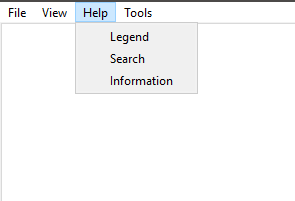
\includegraphics[scale=0.5]{imagini/implementare/helpmenu.png}
    \end{center}
    \caption{Meniul Help}
    \label{fig:tabs}
\end{figure}

\begin{figure}[H]
    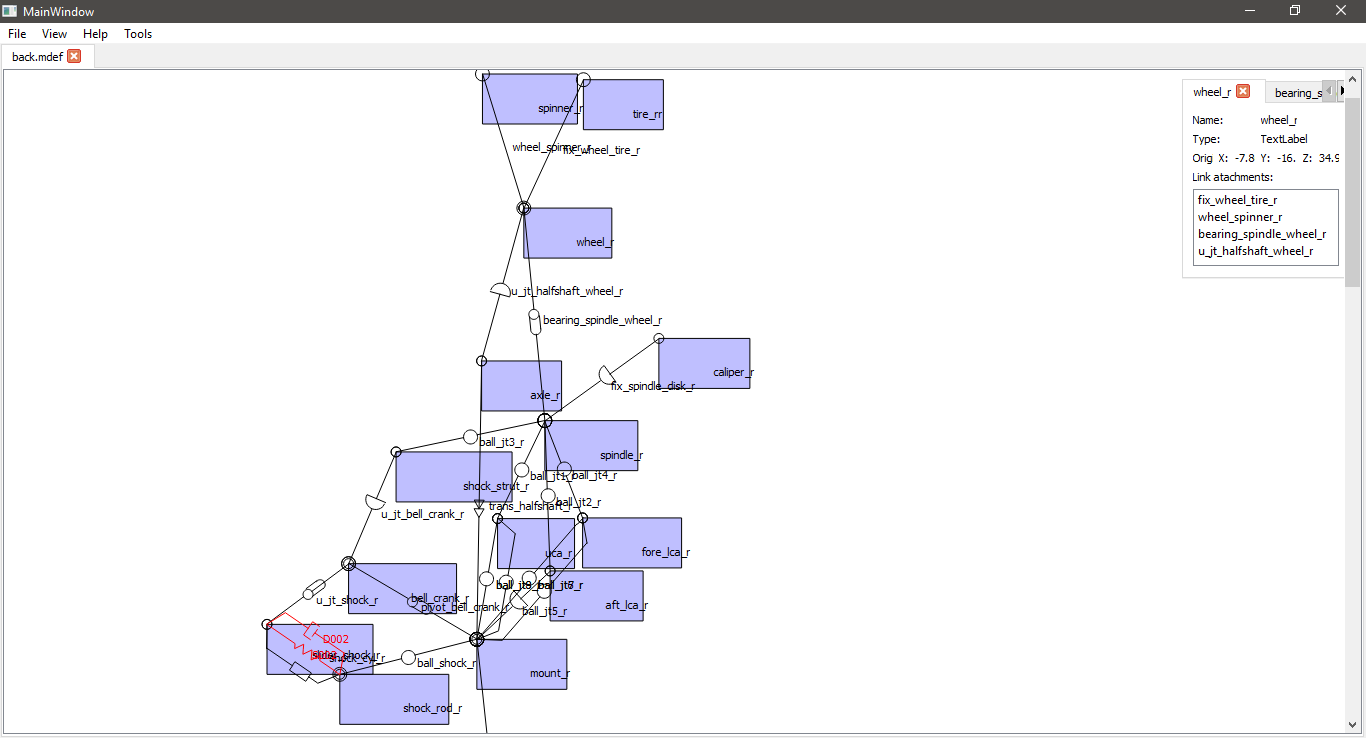
\includegraphics[width=\linewidth]{imagini/implementare/info.png}
    \caption{Panoul cu informații despre un element Motion body}
    \label{fig:tabs}
\end{figure}

\subsection{Legenda}
O alta opțiune de ajutor este cea de legenda. 
Din \verb|help,legend| se deschide un nou panou care afișează toate simbolurile de elemente Joint și elemente Connector pentru ca 
utilizatorul sa înțeleagă mai bine structura modelului.\newline 

\begin{figure}[H]
    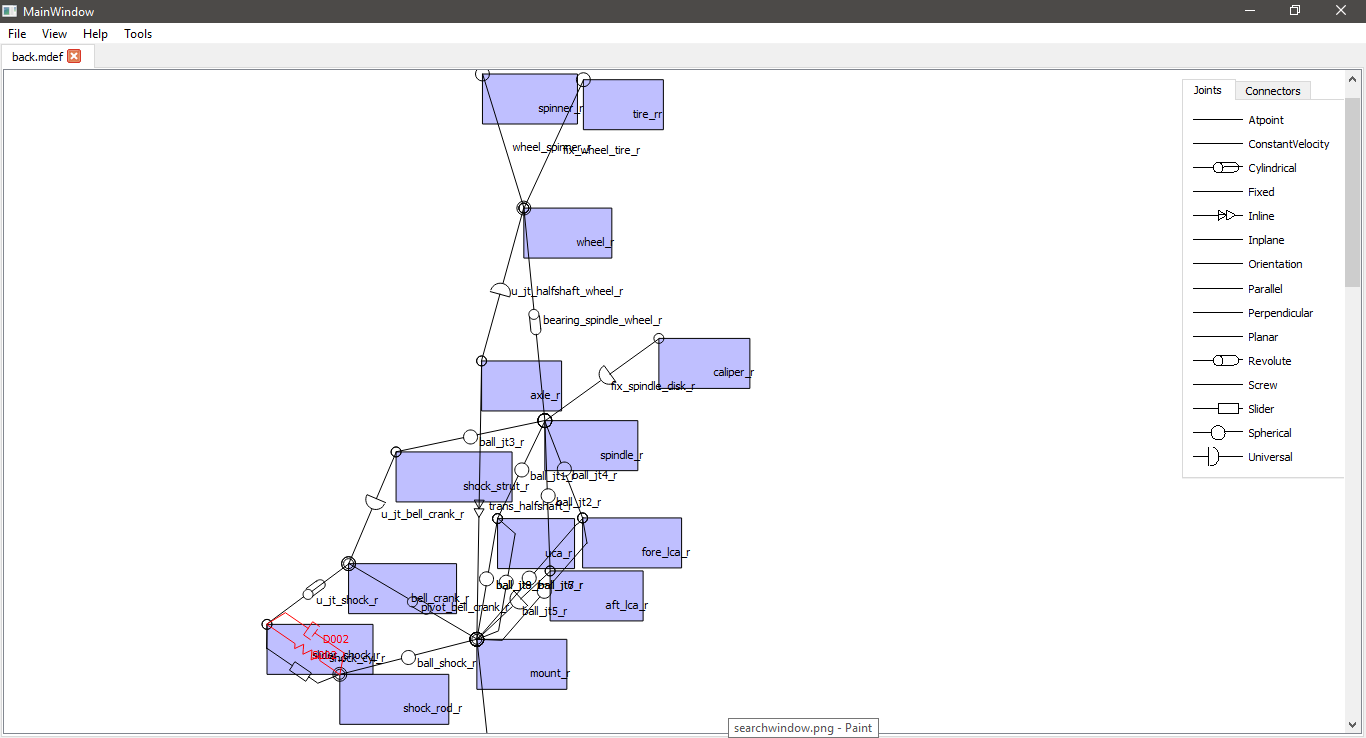
\includegraphics[width=\linewidth]{imagini/implementare/legend.png}
    \caption{Legenda}
    \label{fig:tabs}
\end{figure}

\newpage
\section{Anexa}

\subsection{XML}
\subsubsection{Motion body}
Exemplu simplificat de element care reprezintă un corp de mișcare în fișierul .mdef:
\lstset{language=XML}
\begin{lstlisting}
<MotionBody Name="m1">
    <MassAndInertia>
        <TransformationMatrix>
            <Origin>
                <X Unit="in" Value="-7.58042829409448870592e+00"/>
                <Y Unit="in" Value="4.23044650011811071977e+01"/>
                <Z Unit="in" Value="3.44301163838582695575e+01"/>
            </Origin>
        </TransformationMatrix>
    </MassAndInertia>
</MotionBody>

\end{lstlisting}

\subsubsection{Joint}
Exemplu simplificat de element care reprezintă o legătură între două corpuri de mișcare:

\lstset{language=XML}
\begin{lstlisting}
<Joint Name="u_jt_shock_l" Type="Cylindrical">
    <Action>
        <SelectedMotionBody Name="shock_cyl_l"/>
        <TransformationMatrix>
            <Origin>
                <X Unit="in" Value="-4.14178975641839031141e+00"/>
                <Y Unit="in" Value="2.03613060274620565338e+01"/>
                <Z Unit="in" Value="4.14651875259415945152e+01"/>
            </Origin>
        </TransformationMatrix>
    </Action>
    <Base>
        <SelectedMotionBody Name="bell_crank_l"/>
        <TransformationMatrix>
            <Origin>
                <X Unit="in" Value="-4.14178975641839031141e+00"/>
                <Y Unit="in" Value="2.03613060274620565338e+01"/>
                <Z Unit="in" Value="4.14651875259415945152e+01"/>
            </Origin>
        </TransformationMatrix>
        <SnapMotionBodies Value="false"/>
    </Base>
    <DisplayScale Value="1.00000000000000000000e+00"/>
</Joint>
\end{lstlisting}

\subsubsection{Connector}
Exemplu de element conector de tip arc dintre doua corpuri de miscare:

\lstset{language=XML}
\begin{lstlisting}
<Spring Name="S001" Type="MotionBody">
    <Action>
        <SelectedMotionBody Name="shock_rod_l"/>
        <TransformationMatrix>
            <Origin>
                <X Unit="in" Value="4.97282173372801139521e+00"/>
                <Y Unit="in" Value="2.22172095074280626648e+01"/>
                <Z Unit="in" Value="3.98239507981948648307e+01"/>
            </Origin>
        </TransformationMatrix>
    </Action>
    <Base>
        <SelectedMotionBody Name="shock_cyl_l"/>
        <TransformationMatrix>
            <Origin>
                <X Unit="in" Value="1.13657023776269738846e-01"/>
                <Y Unit="in" Value="2.10778191616462606817e+01"/>
                <Z Unit="in" Value="4.04163897920995651702e+01"/>
            </Origin>
        </TransformationMatrix>
    </Base>
</Spring>
\end{lstlisting}

Tag-urile Action si Base de la elementul Joint și Connector arată corpurile de miscare legate.

Toate elementele au o legătura strânsa iar buna funcționalitate a aplicației tine de structura fișierului.

\subsection{Turtle graphics}
\subsubsection{Desenarea unui cilindru}
\begin{lstlisting}
void JointPainterPathCreator::drawRevolutePath(Turtle & turtle, double length) const
    const double radius = 5;

    turtle.forward((length / 2) - radius);

    turtle.save();
    
    //drawing first circle
    turtle.rotate(M_PI / 2);
    const int nrOfSegments = 32;
    const double angle = 2 * M_PI / nrOfSegments;    
    const double segmentLength = radius*sqrt(2.0 - 2.0*cos(angle));

    for (int i = 0; i < nrOfSegments; i++) {
        turtle.forward(segmentLength);
        turtle.rotate(-angle);
    }

    turtle.load();
    turtle.forward(2 * radius, false);

    //drawing cilinder upper line
    const double cilinderLength=10;

    turtle.forward(cilinderLength, false);

    turtle.rotate(-M_PI / 2);
    turtle.forward(radius, false);

    turtle.rotate(-M_PI / 2);
    turtle.forward(cilinderLength + 3);
    turtle.rotate(M_PI);
    turtle.forward(cilinderLength + 3, false);

    turtle.save();
    for (int i = 0; i < nrOfSegments / 2; i++) {
        turtle.forward(segmentLength);
        turtle.rotate(angle);
    }

    turtle.load();
    turtle.rotate(M_PI / 2);
    turtle.forward(radius*2.0,false);
    turtle.rotate(M_PI / 2);

    //drawing cilinder lower line
    turtle.forward(cilinderLength + 3);
    turtle.rotate(M_PI);
    turtle.forward(cilinderLength + 3, false);
    turtle.rotate(-M_PI);

    turtle.rotate(M_PI / 2);
    turtle.forward(radius, false);

    turtle.rotate(M_PI / 2);
    turtle.forward(radius, false);
}
}
\end{lstlisting}

\newpage
\section{Bibliografie}


\begin{thebibliography}{9}

    \bibitem{topolgy}
    Wikipedia contributors. 
    \textit{Topology}. 
    Wikipedia, The Free Encyclopedia, 2019. 
    \\\texttt{https://en.wikipedia.org/wiki/Topology}

    \bibitem{xml} 
    Bidyottama Koirala.
    \textit{DEVELOPING AN XML-BASED APPLICATION}.  
    Turun Ammattikorkeakoulu, Turku University Of Applied Sciences, 2014.
     
    \bibitem{xml2}
    Wikipedia contributors. 
    \textit{XML}. 
    Wikipedia, The Free Encyclopedia, 2019. 
    \\\texttt{https://en.wikipedia.org/wiki/XML}

    \bibitem{ortographic}
    Dr. Akhilesh Kumar Maurya.
    \textit{ORTHOGRAPHIC PROJECTIONS}.
    Indian Institute Of Technology Guwahati, 2016
    
    \bibitem{ortographic2}
    Wikipedia contributors. 
    \textit{Orthographic projection}. 
    Wikipedia, The Free Encyclopedia, 2019.
    \\\texttt{https://en.wikipedia.org/wiki/Orthographic\_projection}

    \bibitem{turtle}
    Matthias Graf.
    \textit{Direct Manipulation of Turtle Graphics}.
    Otto-von-Guericke University Magdeburg, 2014

    \bibitem{turtle2}
    Wikipedia contributors. 
    \textit{Turtle graphics}. 
    Wikipedia, The Free Encyclopedia, 2019. 
    \\\texttt{https://en.wikipedia.org/wiki/Turtle\_graphics}

    \bibitem{graf}
    J. A. Bondy, U. S. R. Murty.
    \textit{GRAPH THEORY WITH APPLICATIONS}. 
    Department of Combinatorics and Optimization, University of Waterloo, Ontario, Canada, 1976
    
    \bibitem{graf2}
    Wikipedia contributors. 
    \textit{Graph theory}. 
    Wikipedia, The Free Encyclopedia, 2019.
    \\\texttt{https://en.wikipedia.org/wiki/Graph\_theory}
    
    \bibitem{graf3}
    Wikipedia contributors. 
    \textit{Multigraph}. 
    Wikipedia, The Free Encyclopedia, 2019.
    \\\texttt{https://en.wikipedia.org/wiki/Multigraph}

    \bibitem{graf4}
    Slavic Sorin
    \textit{Grafuri Planare}
    Facultatea de Matematică și Informatică, Universitatea din București, 2010

    \bibitem{force}
    Stephen G. Kobourov
    \textit{Force-Directed Drawing Algorithms}
    University of Arizona.

    \bibitem{force2}    
    Wikipedia contributors. 
    \textit{Force-directed graph drawing}. 
    Wikipedia, The Free Encyclopedia, 2019.
    \\\texttt{https://en.wikipedia.org/wiki/Force-directed\_graph\_drawing}

    \bibitem{qt}
    Qt Company.
    \textit{Graphics View Framework}
    \\\texttt{https://doc.qt.io/archives/qt-4.8/graphicsview.html}

    \bibitem{cpp}
    Wikipedia contributors. 
    \textit{C++}. 
    Wikipedia, The Free Encyclopedia, 2019.
    \\\texttt{https://en.wikipedia.org/wiki/C\%2B\%2B}

    \bibitem{qtwiki}
    Wikipedia contributors. 
    \textit{Qt (software)}. 
    Wikipedia, The Free Encyclopedia, 2019.
    \\\texttt{https://en.wikipedia.org/wiki/Qt\_(software)}

    \bibitem{cae}
    Alexander Kolbasin, Oksana Husu.
    \textit{Computer-aided design and Computer-aided engineering}.
    Moscow State University of Civil Engineering, 2018

    \bibitem{cae2}
    \textit{Motion Simulation, Student guide, SC12}.
    Siemens PLM Software, 2018

    

\end{thebibliography}

\end{document}